% allgem. Dokumentenformat
\documentclass[a4paper,12pt,headsepline]{scrartcl}
%Variablen welche innerhalb der gesamten Arbeit zur Verfügung stehen sollen
\newcommand{\titleDocument}{Bachelor Thesis}
\newcommand{\subjectDocument}{in Applied Computer Science}


\newcommand{\specialcell}[2][c]{%
	\begin{tabular}[#1]{c}
		#2
	\end{tabular}
}

\newcommand{\specialcellleft}[2][@{}l]{%
	\begin{tabular}[#1]{@{}l}
		#2
	\end{tabular}
}

\newcommand{\fixme}[1]{
	~\\
	\noindent
	\textbf{\textcolor{red}{FIXME: #1}}
	\\
}




% weitere Pakete
% Grafiken aus PNG Dateien einbinden
\usepackage{graphicx}

% Eurozeichen einbinden
\usepackage[right]{eurosym}

\usepackage{ctable}

% Umlaute unter UTF8 nutzen
\usepackage[utf8]{inputenc}

% Zeichenencoding
\usepackage[T1]{fontenc}

\usepackage{lmodern}
\usepackage{fix-cm}

\usepackage{svg}

% floatende Bilder ermöglichen
%\usepackage{floatflt}

% mehrseitige Tabellen ermöglichen
\usepackage{longtable}

\usepackage{afterpage}

% Unterstützung für Schriftarten
%\newcommand{\changefont}[3]{ 
%\fontfamily{#1} \fontseries{#2} \fontshape{#3} \selectfont}

\setcounter{secnumdepth}{4}
\setcounter{tocdepth}{4}

% Packet für Seitenrandabständex und Einstellung für Seitenränder
\usepackage{geometry}
\geometry{left=3.5cm, right=2cm, top=2.5cm, bottom=2cm}

% Paket für Boxen im Text
\usepackage{fancybox}

% bricht lange URLs "schoen" um
\usepackage[hyphens,obeyspaces,spaces]{url}

% Paket für Textfarben
\usepackage{color}

% Mathematische Symbole importieren
\usepackage{amssymb}

% auf jeder Seite eine Überschrift (alt, zentriert)
%\pagestyle{headings}

% erzeugt Inhaltsverzeichnis mit Querverweisen zu den Kapiteln (PDF Version)
\usepackage[bookmarksnumbered,pdftitle={\titleDocument},hyperfootnotes=false]{hyperref} 
%\hypersetup{colorlinks, citecolor=red, linkcolor=blue, urlcolor=black}
%\hypersetup{colorlinks, citecolor=black, linkcolor= black, urlcolor=black}

% neue Kopfzeilen mit fancypaket
\usepackage{fancyhdr} %Paket laden
\pagestyle{fancy} %eigener Seitenstil
\fancyhf{} %alle Kopf- und Fußzeilenfelder bereinigen
\fancyhead[L]{\nouppercase{\leftmark}} %Kopfzeile links
\fancyhead[C]{} %zentrierte Kopfzeile
\fancyhead[R]{\thepage} %Kopfzeile rechts
\renewcommand{\headrulewidth}{0.4pt} %obere Trennlinie
%\fancyfoot[C]{\thepage} %Seitennummer
%\renewcommand{\footrulewidth}{0.4pt} %untere Trennlinie

% für Tabellen
\usepackage{array}

% Runde Klammern für Zitate
%\usepackage[numbers,round]{natbib}

% Festlegung Art der Zitierung - Havardmethode: Abkuerzung Autor + Jahr
\bibliographystyle{alphadin}

% Schaltet den zusätzlichen Zwischenraum ab, den LaTeX normalerweise nach einem Satzzeichen einfügt.
\frenchspacing

% Paket für Zeilenabstand
\usepackage{setspace}

% für Bildbezeichner
\usepackage{capt-of}

% für Stichwortverzeichnis
\usepackage{makeidx}

% für Listings
\usepackage{listings}
\lstset{numbers=left, numberstyle=\tiny, numbersep=5pt, keywordstyle=\color{black}\bfseries, stringstyle=\ttfamily,showstringspaces=false,basicstyle=\footnotesize,captionpos=b}
\lstset{language=java}

% Indexerstellung
\makeindex

% Abkürzungsverzeichnis
\usepackage[english]{nomencl}
\let\abbrev\nomenclature

% Abkürzungsverzeichnis LiveTex Version
\renewcommand{\nomname}{Abbreviations}
\setlength{\nomlabelwidth}{.25\hsize}
\renewcommand{\nomlabel}[1]{#1 \dotfill}
\setlength{\nomitemsep}{-\parsep}
\makenomenclature
%\makeglossary

% Abkürzungsverzeichnis TeTEX Version
% \usepackage[german]{nomencl}
% \makenomenclature
% %\makeglossary
% \renewcommand{\nomname}{Abkürzungsverzeichnis}
% \setlength{\nomlabelwidth}{.25\hsize}
% \renewcommand{\nomlabel}[1]{#1 \dotfill}
% \setlength{\nomitemsep}{-\parsep}

% Disable single lines at the start of a paragraph (Schusterjungen)
\clubpenalty = 10000
% Disable single lines at the end of a paragraph (Hurenkinder)
\widowpenalty = 10000
\displaywidowpenalty = 10000

\begin{document}
% hier werden die Trennvorschläge inkludiert
%hier müssen alle Wörter rein, welche Latex von sich auch nicht korrekt trennt bzw. bei denen man die genaue Trennung vorgeben möchte
\hyphenation{
Film-pro-du-zen-ten
Lux-em-burg
Soft-ware-bau-steins
zeit-in-ten-siv
}

%Schriftart Helvetica
%\changefont{phv}{m}{n}

% Leere Seite am Anfang
\newpage
\thispagestyle{empty} % erzeugt Seite ohne Kopf- / Fusszeile

% Titelseite %
% das Papierformat zuerst
%\documentclass[a4paper, 11pt]{article}

% deutsche Silbentrennung
%\usepackage[ngerman]{babel}

% wegen deutschen Umlauten
%\usepackage[ansinew]{inputenc}

% hier beginnt das Dokument
%\begin{document}


\thispagestyle{empty}

%\begin{figure}[t]
% \includegraphics[width=0.6\textwidth]{abb/fh_koeln_logo}
%\end{figure}

\begin{figure}[t]
 \centering
 
\includegraphics[width=0.6\textwidth]{abb/logo1}
~~~~~~~~~~
 
\includegraphics[width=0.20\textwidth]{abb/logo2}
\end{figure}


\begin{verbatim}


\end{verbatim}

\begin{center}
\Large{University of Bayreuth}\\
\end{center}


\begin{center}
\Large{Institute for Computer Science}
\end{center}
\begin{verbatim}








\end{verbatim}
\begin{center}
\doublespacing
\textbf{\LARGE{\titleDocument}}\\
\singlespacing
\begin{verbatim}

\end{verbatim}
\textbf{{~\subjectDocument}}
\end{center}
\begin{verbatim}

\end{verbatim}
\begin{center}

\end{center}
\begin{verbatim}






\end{verbatim}
\begin{flushleft}
\begin{tabular}{llll}
\textbf{Topic:} & & Integration of JPA-conform ORM-Implementations & \\
	& & in Hibernate Search & \\
& & \\
\textbf{Author:} & & Martin Braun <martinbraun123@aol.com>& \\
& & Matrikel-Nr. 1249080 & \\
& & \\
\textbf{Version date:} & & \today &\\
& & \\
\textbf{1. Supervisor:} & & Prof. Dr. Stefan Jablonski &\\
\textbf{2. Supervisor:} & & Prof. Dr. Bernhard Westfechtel &\\
\end{tabular}
\end{flushleft}

\pagebreak
~
\pagebreak

\begin{verbatim}






















\end{verbatim}

\begin{center}
	To my parents.
\end{center}

\afterpage{\null\newpage}
\pagebreak
~\\\\
\pagebreak
~


% römische Numerierung
%\pagenumbering{arabic}

% 1.5 facher Zeilenabstand
\onehalfspacing

% Einleitung / Abstract
% !TeX spellcheck = en_GB
\section*{Abstract}\label{abtract}
Every year, lecturer in the field of theoretical computer science or an related one face the task to create an exam exercise that tests if their students have understood the way of working of the Cocke-Younger-Kasami algorithm. Various implementations and small online tools of the CYK algorithm can be found, but none actually assists during the process of creating an exercise.\\
Therefore various algorithms to generate specifically suitable exercises have been designed and compared through their success rates. The different approaches for these algorithms involve the uniform randomly distribution of elements and the general Bottom-Up and Top-Down parsing approaches.\\
A GUI tool to automatically generate these exam exercises has been implemented. Its functionality contains that input parameters such as the count of variables, the count of terminals and the size of the word can be given. Suitable exam exercises are generated and one can be chosen for further modification and creation of the final exam exercise.\\


~~

\section*{Zusammenfassung}\label{zusammenfassung}
Jedes Jahr stehen Dozenten der theoretischen Informatik oder eines verwandten Bereiches vor der Aufgabe Klausuraufgaben zu erstellen, die prüfen ob ihre Studenten die Arbeitsweise des Cocke-Younger-Kasami-Algorithmus verstanden haben. Verschiedene Implementierungen und kleinere Online-Tools des CYK-Algorithmus gibt es bereits, aber Keines unterstützt beim Prozess des Erstellen einer Aufgabe.\\
Verschiedene Algorithmen wurden zuerst entworfen, um genau passende Aufgaben zu generieren und wurden anschließend auch miteinander über ihre Erfolgsrate verglichen. Die unterschiedlichen Ansätze für die Algorithmen beinhalten das gleichmäßig zufällige Verteilen von Elementen und die allgemeinen Ansätze des Bottom-Up und Top-Down Parsings.\\
Es wurde ein GUI-Tool implementiert um automatisch Klausuraufgaben zu generieren. Die Funktionalität des Tools beinhaltet, dass Eingabewerte wie die Anzahl der Variablen, die Anzahl der Terminale und die Wortlänge gemacht werden können. Geeignete Klausuraufgaben werden automatisch generiert von denen Eine für weitere Modifikation und letztendlich für die Klausuraufgabenerstellung ausgewählt wird.\\



\pagebreak



% einfacher Zeilenabstand
\singlespacing

% Inhaltsverzeichnis anzeigen
\newpage
\tableofcontents
~
\pagebreak

% das Abbildungsverzeichnis
%\newpage
% Abbildungsverzeichnis soll im Inhaltsverzeichnis auftauchen
%\addcontentsline{toc}{section}{List of figures}
% Abbildungsverzeichnis endgueltig anzeigen
%\listoffigures

% das Tabellenverzeichnis
%\newpage
% Abbildungsverzeichnis soll im Inhaltsverzeichnis auftauchen
%\addcontentsline{toc}{section}{Tabellenverzeichnis}
% \fancyhead[L]{Abbildungsverzeichnis / Abkürzungsverzeichnis} %Kopfzeile links
% Abbildungsverzeichnis endgueltig anzeigen
%\listoftables

%% WORKAROUND für Listings
%\makeatletter% --> De-TeX-FAQ
%\renewcommand*{\lstlistoflistings}{%
%  \begingroup
%    \if@twocolumn
%      \@restonecoltrue\onecolumn
%    \else
%      \@restonecolfalse
%    \fi
%    \lol@heading
%    \setlength{\parskip}{\z@}%
%    \setlength{\parindent}{\z@}%
%    \setlength{\parfillskip}{\z@ \@plus 1fil}%
%    \@starttoc{lol}%
%    \if@restonecol\twocolumn\fi
%  \endgroup
%}
%\makeatother% --> \makeatletter
% das Listingverzeichnis
%\newpage
% Listingverzeichnis soll im Inhaltsverzeichnis auftauchen
%\addcontentsline{toc}{section}{Listingverzeichnis}
%\fancyhead[L]{Abbildungs- / Tabellen- / Listingverzeichnis} %Kopfzeile links
%\renewcommand{\lstlistlistingname}{Listingverzeichnis}
%\lstlistoflistings
%%%%

% das Abkürzungsverzeichnis
%\newpage
% Abkürzungsverzeichnis soll im Inhaltsverzeichnis auftauchen
%\addcontentsline{toc}{section}{Abkürzungsverzeichnis}
% das Abkürzungsverzeichnis entgültige Ausgeben
%\fancyhead[L]{Abkürzungsverzeichnis} %Kopfzeile links
%\nomenclature{UGC}{User Generated Content}
\nomenclature{CSS}{Cascading Style Sheets}
\nomenclature{JS}{JavaScript}
\nomenclature{SQL}{Structured Query Language}
\nomenclature{GPL}{GNU General Public License}
\nomenclature{GNU}{GNU is not Unix}
\nomenclature{LGPL}{GNU Lesser General Public License}
\nomenclature{XMPP}{Extensible Messaging and Presence Protocol}
\nomenclature{IM}{Instant Message}
\nomenclature{CMS}{Content Management System}
\nomenclature{RSS}{Really Simple Syndication}
\nomenclature{JSON}{JavaScript Object Notation}
\nomenclature{HTML}{Hypertext Markup Language}
\nomenclature{TDD}{Test-driven development}
\nomenclature{GUI}{Graphical User Interface}
\nomenclature{KPI}{Key Performance Indicator}
\nomenclature{WWW}{World Wide Web}
\nomenclature{OCR}{Optical Character Recognition}
\nomenclature{ERM}{Entity Relationship Modell}

%\printnomenclature

% Definiert Stegbreite bei zweispaltigem Layout
\setlength{\columnsep}{25pt}

%%%%%%% EINLEITUNG %%%%%%%%%%%%
%\twocolumn
\newpage
\fancyhead[L]{\nouppercase{\leftmark}} %Kopfzeile links

% 1,5 facher Zeilenabstand
\onehalfspacing

% einzelne Kapitel
% !TeX spellcheck = en_GB

\section{Introduction}\label{Introduction}

\noindent What has already been done in this area? Why are you doing this?\\ 

\noindent Let there be a grammar $G=(V,\ \Sigma,\ S,\ P)$ in Chomsky Normal Form (CNF).\\
$V$ is a finite set of variables. \\
$\Sigma$ is an alphabet. \\
$S$ is the starting symbol and $S \in V$. \\
$P$ is a finite set of rules: $P \subseteq V \times (V \cup \Sigma)^{*}$. $G$ is in CNF and therefore, more specifically, it holds:  $P\ \subseteq\ V \times (V^{2} \cup \Sigma)$.\\
 
\noindent For simplification the default definitions hold:
\begin{itemize}
	\item $V = \{A, B, ...\}$
	\item $(V^2 \cup\ \Sigma)^{*}=\{a, b, ...\} \cup \{AB, BS, AC, ... \}$
\end{itemize}

\noindent Let there be a word $w \in \Sigma^*$, a language $L(G)$ and a grammar $G$ in CNF. 

\subsection{Forward Problem vs. Backward Problem}

\noindent\textbf{Forward Problem ($G \xrightarrow[]{derivation} w$):}\\
Informal definition: "Forming a derivation from a root node to a final sentence."  [Duda 8.6.3 page 426]\\
Input: Grammar $G$ in CNF.\\
Output: Derivation $d$ that shows implicitly $w \subseteq L$.\\

\noindent\textbf{Backward Problem = Parsing ($w\overset{?}{\subseteq}L(G)$):}\\
Informal definition: "Given a particular $w$, find a derivation in $G$ that leads to $w$. This process, called parsing, is virtually always much more difficult than forming a derivation."  [Duda 8.6.3 page 426]\\
Input: $w$ and a grammar $G$ in CNF.\\
Output: $w \subseteq L(G) \Longrightarrow$ derivation $d$.\\

\subsection{Parsing: Bottom-Up vs Top-Down}

\noindent\textbf{Bottom-Up:} Bottom-Up parsing is "the general method used in the Cocke-Younger-Kasami(CYK) algorithm, which fills a parse table from the "bottom up"." (Bottom up means starting from the leaves.) [Duda 8.6.3 page 426]\\

\noindent\textbf{Top-Down:} "Top-Down parsing starts with the root node and successively applies productions from $P$, with the goal of finding a derivation of the test sentence $w$. Because it is rare indeed that the sentence is derived in the first production attempted, it is necessary to specify some criteria to guide the choice of which rewrite rule to apply. Such criteria could include beginning the parse at the first (left) character in the sentence (i.e., finding a small set of rewrite rules that yield the first character), then iteratively expanding the production to derive subsequent characters, or instead starting at the last (right) character in the sentence." [Duda 8.6.3 page 428]\\

\subsection{Scope of this thesis}

The starting point of this thesis was to get a command line interface (CLI) tool to automatically generate $exercises = (grammar,\ word,\ parse\ table,\ derivation\ tree)$, which are used to test if the students have understood the way of working of the CYK algorithm. A scoring model is used to evaluate the generated exercises regarding their usability in an exam.\\

\noindent This alone doesn't meet the requirements for being an adequate topic for a bachelor thesis.
Therefore the task of finding a clever algorithm to get exercises with a high chance of being usable as an exam exercise was added.\\

\pagebreak

% !TeX spellcheck = en_GB

\section{Technology Overview}\label{TechnologyOverview}

\pagebreak

% !TeX spellcheck = en_GB

~
\pagebreak

\section{Challenges}\label{Challenges}
While building the generic version of Hibernate Search, we will encounter some challenges. First, we will introduce a small example project. We will then use this project to illustrate the biggest challenges. It will also be used to showcase some problems and usages later on in this thesis.

\subsection{The example project} \label{example_project}
Consider a software built with JPA that is used to manage the inventory of a bookstore. It stores information about the available books (ISBN, title, genre, short summary of the contents) and the corresponding authors (surrogate id, first \& last name, country) in a relational database. Each author is related to zero or more Books and each Book is written by one or more Authors. The entity relationship model diagram defining the database looks like this:
\\
\begin{figure}[ht]
	\centering
	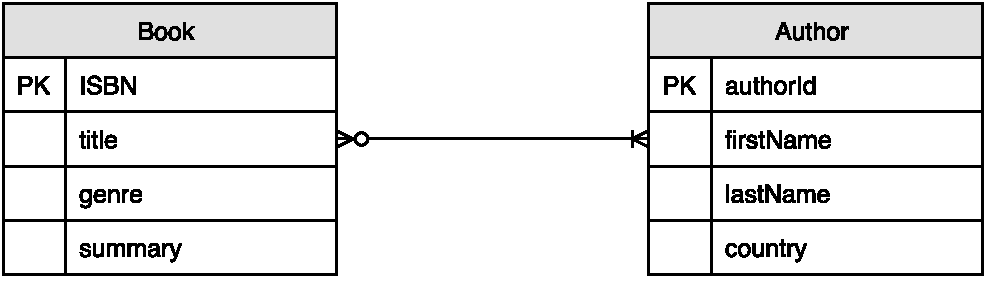
\includegraphics[scale = 0.9]{images/Sample_Project_ER.pdf}
	\caption{the bookstore entity relationship model}
	\label{fig3}
\end{figure}
\\
Using a mapping table for the M:N relationship of Author and Book, the database contains three tables: Author, Book and Author\_Book. The applications strictly uses JPA to access the data without any vendor specific features. The JPA annotated classes for these entities are defined as shown in the following listings.

\pagebreak

\lstset{language=java}
\begin{lstlisting}[frame=htrbl, caption={Book.java}, label={lst:book.java_1}]
@Entity
@Table(name = "Book")
public class Book {

	@Id
	@Column(name = "isbn")
	private String isbn;
	
	@Column(name = "title")
	private String title;
	
	@Column(name = "genre")
	private String genre;
	
	@Lob
	@Column(name = "summary")
	private String summary;
	
	@ManyToMany(mappedBy = "books", cascade = {
		CascadeType.MERGE,
		CascadeType.DETACH,
		CascadeType.PERSIST,
		CascadeType.REFRESH
	})
	private Set<Author> authors;
	
	//getters & setters ...
}
\end{lstlisting}

\pagebreak

\lstset{language=java}
\begin{lstlisting}[frame=htrbl, caption={Author.java}, label={lst:author.java_1}]
@Entity
@Table(name = "Author")
public class Author {
	
	@Id
	@GeneratedValue(strategy = GenerationType.AUTO)
	@Column(name = "authorId")
	private Long authorId;
	
	@Column(name = "firstName")
	private String firstName;
	
	@Column(name = "lastName")
	private String lastName;
	
	@Column(name = "country")
	private String country;
	
	@ManyToMany(cascade = {
		CascadeType.MERGE, 
		CascadeType.DETACH, 
		CascadeType.PERSIST, 
		CascadeType.REFRESH
	})
	@JoinTable(name = "Author_Book", 
		joinColumns = 
			@JoinColumn(name = "authorFk", 
				referencedColumnName = "authorId"),
		inverseJoinColumns = 
			@JoinColumn(name = "bookFk", 
				referencedColumnName = "isbn"))
	private Set<Book> books;
	
	//getters & setters ...
}
\end{lstlisting}
For the sake of simplicity and since every JPA provider is able to derive a default DDL script from the annotations, we don't supply any information about how to create the database schema here. However, for real world applications defining a hand-written DDL script might be a better idea since the generated code might not be optimal and could differ between the different JPA implementations and RDBMSs used.

\pagebreak

\subsection{Standalone version} \label{problem_indexing_searching}
Hibernate Search's engine wasn't designed to be used directly by application developers. Its main purpose is to serve as an integration point for other APIs that need to leverage its power to index object graphs and query the index for hits by exposing a quite low-level and in some ways complex API. This is why we have to write our own standalone version based on the "hibernate-search-engine" serving as an abstraction layer such that it eases the usage of the engine in our JPA integration.

\subsection{JPA integration}
After the standalone version is finished, we will build an integration of it with JPA. By incorporating the same engine that the original does, we will support the same indexing behaviour and even stay compatible with entities designed for the original with as little changes as possible. In fact, the main goal for the JPA integration is to be as compatible as possible with Hibernate Search ORM.
\\\\\
The implementations of these two challenges are represented by the modules "Hibernate Search Standalone" and "Hibernate Search GenericJPA" in the following figure \ref{hibernate_search_genericjpa_complete_architecture}. Together with the module "Hibernate Search Database Utilities", these are the submodules of our complete generic version and the result of the top-bottom analysis as described in chapter \ref{Methods}. Note that during this thesis we will be referring to the whole project by the name of the main module "Hibernate Search GenericJPA" as well.

\begin{figure}[ht]
	\centering
	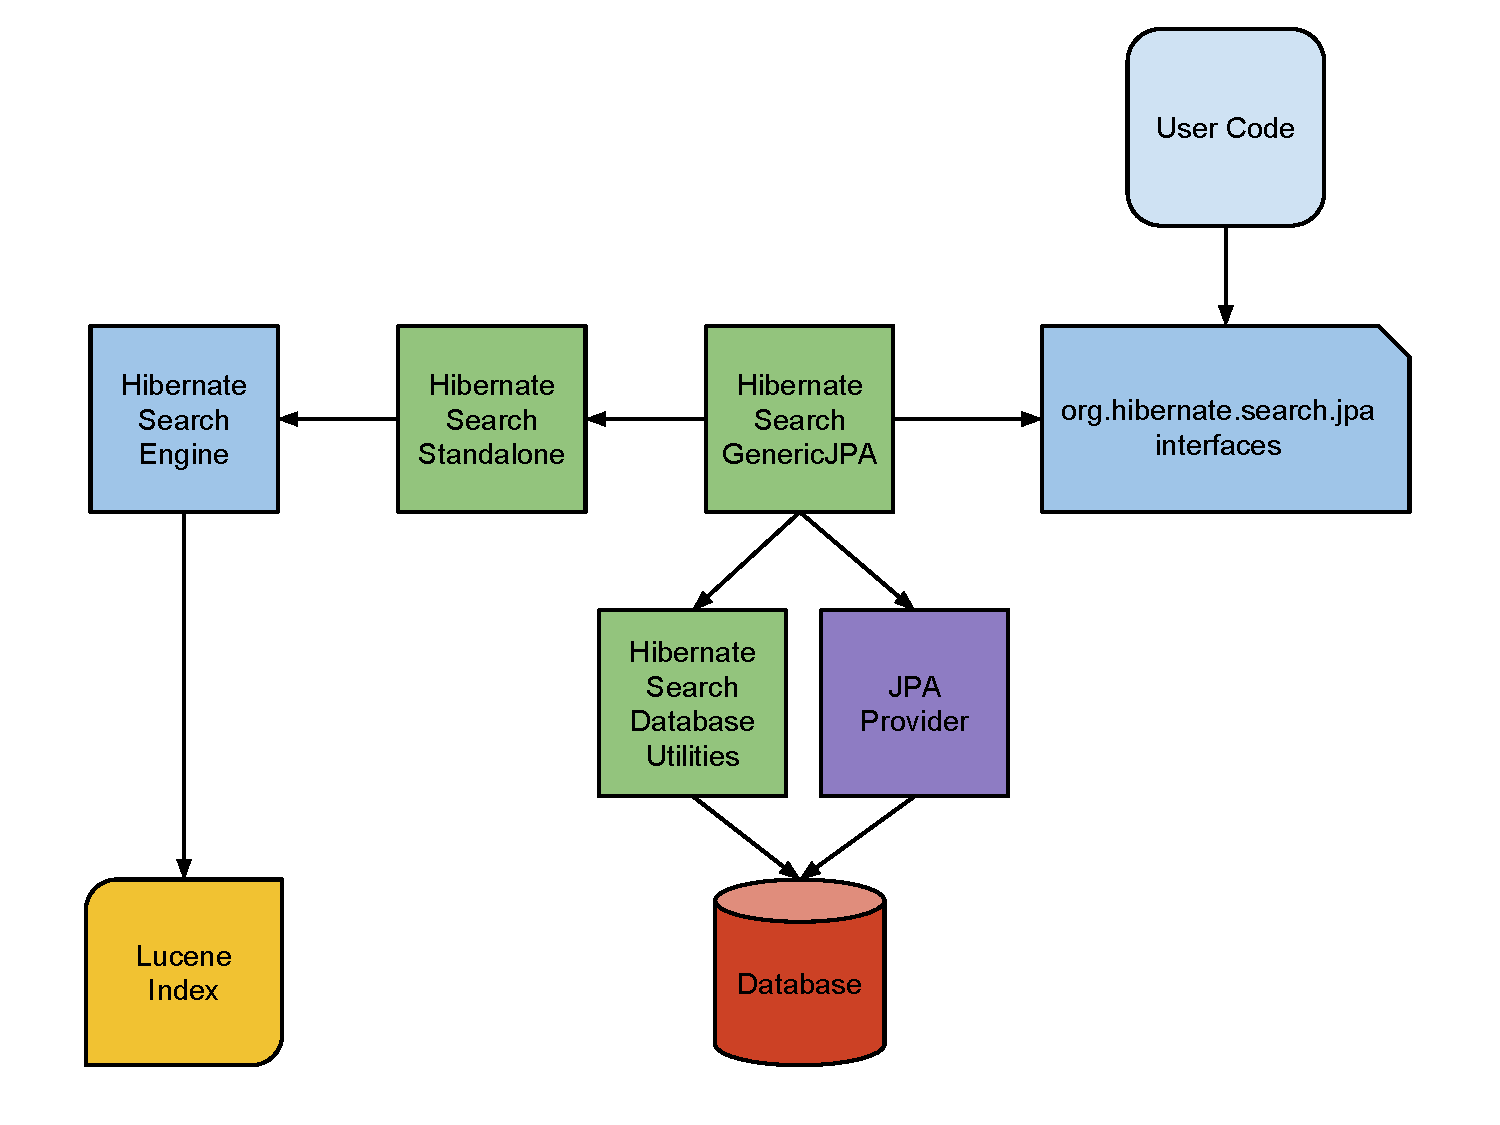
\includegraphics[scale=0.5]{images/hibernate_search_genericjpa_complete_architecture.pdf}
	\caption{Complete Architecture of Hibernate Search GenericJPA}
	\label{hibernate_search_genericjpa_complete_architecture}
\end{figure}

\pagebreak

%\subsection{Index rebuilding}
%If the way objects are indexed changes, the existing files have to %be purged and recreated in the new index format. The naive approach %here would be purging the index and then indexing all data %sequentially as they are retrieved from the database:
%\\
%\lstset{language=java}
%\begin{lstlisting}[frame=htrbl, caption={naive index rebuilding}, %label={lst:naiveIndexing}]
%EntityManager em = ...;
%<Hibernate Search Controller> search = ...;
%
%search.purgeAll(Book.class);
%
%Query query = em.createQuery("SELECT b FROM Book b");
%List<Book> booksFromDb = query.getResultList();
%for(Book b : booksFromDb) {
%	search.index(b);
%}
%\end{lstlisting}
%While this might work for small databases, bigger datasets will %cause this algorithm to run out of memory, since we just retrieve %all the data at once. This could be fixed by implementing a %batching strategy, but it would still be quite slow as it only uses %one thread which would mostly be used for I/O from the database.
%\\\\
%This is not optimal, since a index rebuild should be as fast as %possible as the application cannot be properly used while the job %is running. Therefore we need to create a parallel indexing %mechanism, just like the one Hibernate Search ORM has.

\subsection{Automatic index updating} \label{automatic_indexing_problematic_intro}
The most important feature to be re-built, is automatic index updating. In Hibernate Search ORM, every change in the database is automatically reflected in the index. It is important to have this feature, because otherwise developers would have to manually make sure the index is always up-to-date. With bigger project sizes it gets increasingly harder to keep track of all the locations in the code that change index relevant data and inconsistencies in the indexing logic become nearly unavoidable. While this problem might be mitigated by hiding all the database access logic behind a service layer, even such a solution would be hard to keep error-free as for big applications this layer will probably have multiple critical indexing relevant spots as well.
\\\\
The original Hibernate Search ORM is achieving an up-to-date index by listening to specific Hibernate ORM events for all of the C\_UD (CREATE, UPDATE, DELETE) actions. These events also cover entity relationship collections (for example represented by mapping tables like Author\_Book). As our goal is to create a generic Hibernate Search engine that works with any JPA implementation, we cannot rely on any vendor specific event system. Thus, at least an additional generic solution has to be found.
\\\\
This feature will be part of the "Hibernate Search GenericJPA" module.

\subsection{Timeline}
The solutions for the challenges depend on each other in the same order they were described above: the JPA integration can only be worked on as soon as the standalone integration is done and work on the automatic updating mechanism cannot be started without knowing the JPA integration interfaces. The timeline of our project therefore looks like this:
\\
\begin{figure}[ht]
	\centering
	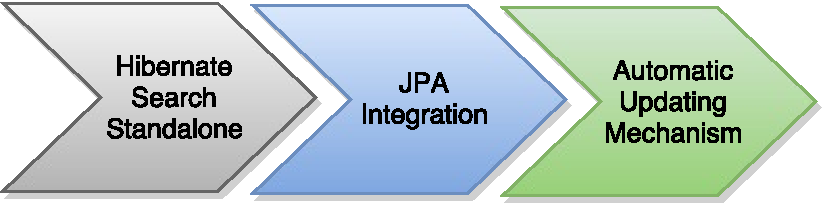
\includegraphics[scale=0.75]{images/timeline_genericjpa_complete.pdf}
	\caption{Timeline of the project}
	\label{project_timeline}
\end{figure}

\pagebreak

% !TeX spellcheck = en_GB

~
\pagebreak

\section{Standalone version of Hibernate Search} \label{standalone_chapter}

\begin{figure}[ht]
	\centering
	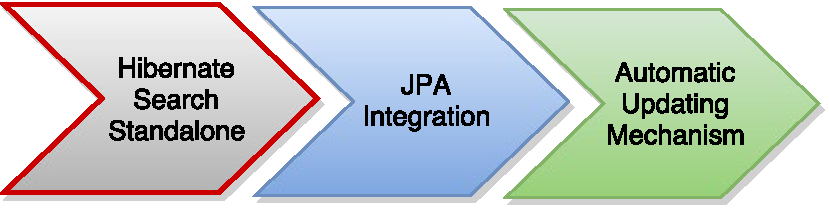
\includegraphics[scale=0.75]{images/timeline_genericjpa_first.pdf}
	\label{project_timeline_first}
\end{figure}
\noindent
We will start the development part of this thesis by discussing how Hibernate Search's engine (in the form of the module "hibernate-search-engine") can be used in general. After this is done we will work out a standalone version of this engine that is easier to work with so we can integrate this standalone version with JPA in the next chapter.
\\\\
As already described earlier in chapter \ref{problem_indexing_searching}, hibernate-search-engine is not intended to be used by application developers, but for other APIs to integrate with. Therefore there is no real public documentation available on how to use it besides the internal JavaDocs \footnote{Hibernate Search JavaDoc, see~\cite{hibernate_search_javadoc}} (describing the classes, but not the interaction between them). Nearly all the following information had to be retrieved from tests in the hibernate-search-engine and hibernate-search-orm integration module source code \footnote{Hibernate Search GitHub, see~\cite{hsearch_source_code_git}}.

\pagebreak

\subsection{Example project with Hibernate Search annotations} \label{setting_up_example_project}

Before we explain how we do things in particular, we set up the example entities described in \ref{example_project} as if the original Hibernate Search would have been used. We do so by adding additional annotations to our entity-classes (only the basic properties are explained here):

\begin{enumerate}
	\item \textbf{@Indexed}: marks the entity as an index root-type.
	\item \textbf{@DocumentId}: marks the field as the id of this entity. this is only needed if no JPA @Id can be found, but can be used to override settings. A Field marked with this
	is stored and indexed. Storing means that its contents are obtainable by projection when retrieving results. This is needed for ids so that the original Entity can be obtained from the database.
	\item \textbf{@Field}: describes how the annotated field should be indexed:
	\\\textbf{@Field\#store} determines whether the contents of this Java property should be stored in the index (Store.YES) or not (Store.NO, default) while \textbf{@Field\#index} determines whether it should be searchable in the index (Index.YES, default) or not (Index.NO). 
	\\
	The index fieldname defaults to the Java property name but can manually be overridden with \textbf{Field\#name} if needed.
	\item \textbf{@IndexedEmbedded}: marks properties that point to other classes which should be included in the index. By default, all fields contained in these entities are prefixed with the property name this is placed on. \\
	\textbf{@IndexedEmbedded\#includeEmbeddedObjectId} decides whether the ids of the embedded objects have to be stored and indexed as well.
	\item \textbf{@ContainedIn}: used in entities that are embedded in other indexes. this is set on the properties that point back to the index-owning entity.
\end{enumerate}
\noindent
As these annotations are defined in hibernate-search-engine, we can rely on all of them while designing the standalone version of Hibernate Search and all other modules depending on it.

\pagebreak
\noindent
The resulting entities look like this:
\\
\lstset{language=java}
\lstset{moredelim=[is][\bfseries]{[*}{*]}}
\begin{lstlisting}[frame=htrbl, caption={Book.java with Hibernate Search annotations}, label={lst:book.java_2}]
@Entity
@Table(name = "Book")
[*@Indexed*]
public class Book {

	@Id
	@Column(name = "isbn")
	[*@DocumentId*]
	private String isbn;
	
	@Column(name = "title")
	[*@Field(store = Store.YES, index = Index.YES)*]
	private String title;
	
	@Column(name = "genre")
	[*@Field(store = Store.YES, index = Index.YES)*]
	private String genre;
	
	@Lob
	@Column(name = "summary")
	[*@Field(store = Store.NO, index = Index.YES)*]
	private String summary;
	
	@ManyToMany(mappedBy = "books", cascade = {
		CascadeType.MERGE,
		CascadeType.DETACH,
		CascadeType.PERSIST,
		CascadeType.REFRESH
	})
	[*@IndexedEmbedded(includeEmbeddedObjectId = true)*]
	private Set<Author> authors;
	
	//getters & setters ...
}
\end{lstlisting}

\pagebreak

\lstset{language=java}
\lstset{moredelim=[is][\bfseries]{[*}{*]}}
\begin{lstlisting}[frame=htrbl, caption={Author.java with Hibernate Search annotations}, label={lst:author.java_2}]
@Entity
@Table(name = "Author")
public class Author {

	@Id
	@GeneratedValue(strategy = GenerationType.AUTO)
	@Column(name = "authorId")
	[*@DocumentId*]
	private Long authorId;
	
	@Column(name = "firstName")
	[*@Field(store = Store.YES, index = Index.YES)*]
	private String firstName;
	
	@Column(name = "lastName")
	[*@Field(store = Store.YES, index = Index.YES)*]
	private String lastName;
	
	@Column(name = "country")
	[*@Field(store = Store.YES, index = Index.YES)*]
	private String country;
	
	@ManyToMany(cascade = {
		CascadeType.MERGE, 
		CascadeType.DETACH, 
		CascadeType.PERSIST, 
		CascadeType.REFRESH
	})
	@JoinTable(name = "Author_Book", 
		joinColumns = 
			@JoinColumn(name = "authorFk", 
				referencedColumnName = "authorId"),
		inverseJoinColumns = 
			@JoinColumn(name = "bookFk", 
				referencedColumnName = "isbn"))
	[*@ContainedIn*]
	private Set<Book> books;
	
	//getters & setters ...
}
\end{lstlisting}

\pagebreak

\subsection{Usage of Hibernate Search's engine} \label{using_hsearch_engine}
In this chapter we will take a look at how to use Hibernate Search's engine natively by showing how it's started, how the index is manipulated and how searching works.

\subsubsection{Startup}
A Hibernate Search engine instance is represented by a \textbf{SearchIntegrator} object. In order to obtain it, we first have to write a special configuration class that implements \textbf{org.hibernate.search.cfg.spi.SearchConfiguration}. An object of this class has then to be created and filled with all the configuration properties Hibernate Search requires. The minimum that has to be set for this to work are the following:

\begin{enumerate}
	\item \textbf{hibernate.search.default.directory\_provider}: The two most common cases here are either "ram" or "filesystem". This decides where the index will be stored. A ram directory is only present in the system memory while the SearchIntegrator exists. A "filesystem" directory is persisted on the hard disk. For "filesystem" the additional property "hibernate.search.default.indexBase" has to be set to an appropriate path.
	
	\item \textbf{hibernate.search.lucene\_version}: This decides which Lucene version has to be used internally. The currently latest supported version supported is "5.2.1" as we are using an early alpha version of Hibernate Search for development (see "Used software" in the appendix). It can be set to earlier versions to support legacy behaviour in some Lucene classes.
\end{enumerate}
\noindent
A complete list of the available settings can be found in the Hibernate Search documentation \footnote{Hibernate Search documentation, see~\cite{hibernate_search_doc}} (only the Hibernate ORM specific settings cannot be used). Our \textbf{StandaloneSearchConfiguration} (appendix listing \ref{lst:StandaloneSearchConfiguration.java}) defaults to "ram" and "5.2.1".

\pagebreak
\noindent
Having this class in place, a \textbf{SearchIntegrator} can be obtained by a \textbf{SearchIntegratorBuilder} like this:
\\
\lstset{language=java}
\lstset{moredelim=[is][\bfseries]{[*}{*]}}
\begin{lstlisting}[frame=htrbl, caption={Starting up the engine}, label={lst:starting_up_engine.java}]
List<Class<?>> indexClasses = Arrays.asList(Book.class, Author.class);

SearchConfiguration searchConfiguration = 
	new StandaloneSearchConfiguration();
indexClasses.forEach( searchConfiguration::addClass );

//bootstrapping class for Hibernate Search
SearchIntegratorBuilder builder = new SearchIntegratorBuilder();

//we have to build an integrator here (the builder needs a 
//"base integrator" first before we can add index classes)
builder.configuration( searchConfiguration ).buildSearchIntegrator();

indexClasses.forEach( builder::addClass );

//starts the engine with all configuration properties set
SearchIntegrator searchIntegrator = builder.buildSearchIntegrator();

//use the integrator ...

//close it
searchIntegrator.close();
\end{lstlisting}

\pagebreak

\subsubsection{Index manipulation} \label{index_manipulation_integrator}

Now that we know how a SearchIntegrator can be built, we can take a look at how we can control the index using the engine's features. 
\\\\
The engine does a lot of optimizations in the backend. This is the reason the specifics are hidden behind a \textbf{Worker} pattern. Such a worker batches operations by synchronizing upon the \textbf{org.hibernate.search.backend.TransactionContext} interface. Our implementation of this is simply called \textbf{Transaction} (appendix listing \ref{lst:Transaction.java}). The different index operations are represented by \textbf{Work} objects that contain the WorkType (INDEX, UPDATE, PURGE, etc.) and all necessary data to execute the individual task.
\\\\
Indexing objects with \textbf{WorkType.INDEX}:
\\
\lstset{language=java}
\begin{lstlisting}[frame=htrbl, caption={Indexing an object with the engine}, label={lst:indexing_object_native.java}]
Book book = ...;
Transaction tx = new Transaction();
Worker worker = searchIntegrator.getWorker();
worker.performWork( new Work( book, WorkType.INDEX ), tx );
tx.commit();
\end{lstlisting}

\noindent
Updating objects with \textbf{WorkType.UPDATE}:
\\
\lstset{language=java}
\begin{lstlisting}[frame=htrbl, caption={Updating an object with the engine}, label={lst:updating_object_native.java}]
Book book = ...;
Transaction tx = new Transaction();
Worker worker = searchIntegrator.getWorker();
worker.performWork( new Work( book, WorkType.UPDATE ), tx );
tx.commit();
\end{lstlisting}
~\\
Deleting objects with \textbf{WorkType.PURGE}:
\\
\lstset{language=java}
\begin{lstlisting}[frame=htrbl, caption={Deleting an object by id with the engine}, label={lst:deleting_object_native.java}]
String isbn = ...;
Transaction tx = new Transaction();
Worker worker = searchIntegrator.getWorker();
worker.performWork( new Work( Book.class, isbn, WorkType.PURGE ), tx );
tx.commit();
\end{lstlisting}

\pagebreak
\noindent
This API doesn't have any "convenience" methods that wrap around the Transaction management if no batching is needed, nor does it have any wrapper utility for the Work object generation.

\subsubsection{Queries}
Querying the index is already acceptable to some extent when it comes to building the actual query. This is mainly due to the fact the query class \textbf{HSQuery} supports method chaining and that the same query builder DSL (which returns Lucene queries) used in Hibernate Search ORM is available. Any basic Lucene query could be used as well, but would require manual analysis of the input. Queries produced by the builder are automatically analysed with the correct Analyzer.
\\
\lstset{language=java}
\lstset{moredelim=[is][\bfseries]{[*}{*]}}
\begin{lstlisting}[frame=htrbl, caption={Querying the index with the engine}, label={lst:querying_natively.java}]
SearchIntegrator searchIntegrator = ...;

[*HSQuery*] query = searchIntegrator.createHSQuery();

//find information about all the entities matching a given title
[*List<EntityInfo>*] entityInfos = 
	query.luceneQuery(
			//query DSL:
			searchIntegrator.buildQueryBuilder()
				.forEntity( Book.class )
				.get()
				.keyword()
				.onField( "title" )
				.matching( "searchString" )
				.createQuery()
		).targetedEntities(
			Collections.singletonList(
				Book.class
			)
		)[*.projection(
			ProjectionConstants.ID
		)*].queryEntityInfos();
\end{lstlisting}

\pagebreak
\noindent
Executing the queries doesn't return anything resembling the original Java objects, though. The actual data returned depends on what we project upon in the projection(...) call and is wrapped in an \textbf{EntityInfo} object. In our example we only retrieve the ids of the Books matching our query. We do this because when using a search index, we don't generally want to work with the actual data found in the index after the hits have been found. We want objects retrieved from the database.
\\
\lstset{language=java}
\begin{lstlisting}[frame=htrbl, caption={Extracting info from the results}, label={lst:querying_natively.java_2}]
//a JPA EntityManager
EntityManager em = ...;

//extract info from the entityInfos
for(EntityInfo entityInfo : entityInfos) {
	String isbn = (String) entityInfo.getProjection()[0];
	//retrieve an object from the database
	Book book = em.find(Book.class, isbn);
	//handle this information ...
}
\end{lstlisting}

\pagebreak
~
\pagebreak

\subsection{Design of the standalone version} \label{standalone_hibernate_search}

In \ref{using_hsearch_engine} we described how the engine can be used natively without any notion of JPA. While using the engine this way is possible, it is not convenient because some of the code is quite complicated. This is the reason we will now discuss a standalone abstraction of this code.
\\\\
As we have seen in the examples earlier, the main interfaces used for index control and querying are \textbf{SearchIntegrator} and \textbf{HSQuery}. In order to abstract some of the complicated logic, we now introduce two new interfaces: 

\begin{itemize}
	\item \textbf{StandaloneSearchFactory}: This interface is responsible for all index changes. Code using this abstraction doesn't have to cope with the Worker pattern, at all. This is hidden behind index/delete/update methods.
	
	\item \textbf{HSearchQuery}: While still having the same chaining methods as HSQuery, we retrieve results from the index in a different manner now. Instead of manually having to extract the ID out of the EntityInfos, this interface retrieves the actually wanted data with the help of the \textbf{EntityProvider} interface which wraps the access to the database. The specifics of the EntityProvider are still use-case specific as the examples later in this chapter will show.
\end{itemize}

\pagebreak

\noindent
The following diagram shows the rough architecture of our new standalone version. Note that we are using a specialization of \textbf{SearchIntegrator} - namely \textbf{ExtendedSearchIntegrator} - which allows us to have more sophisticated features.
\\
\begin{figure}[ht]
	\centering
	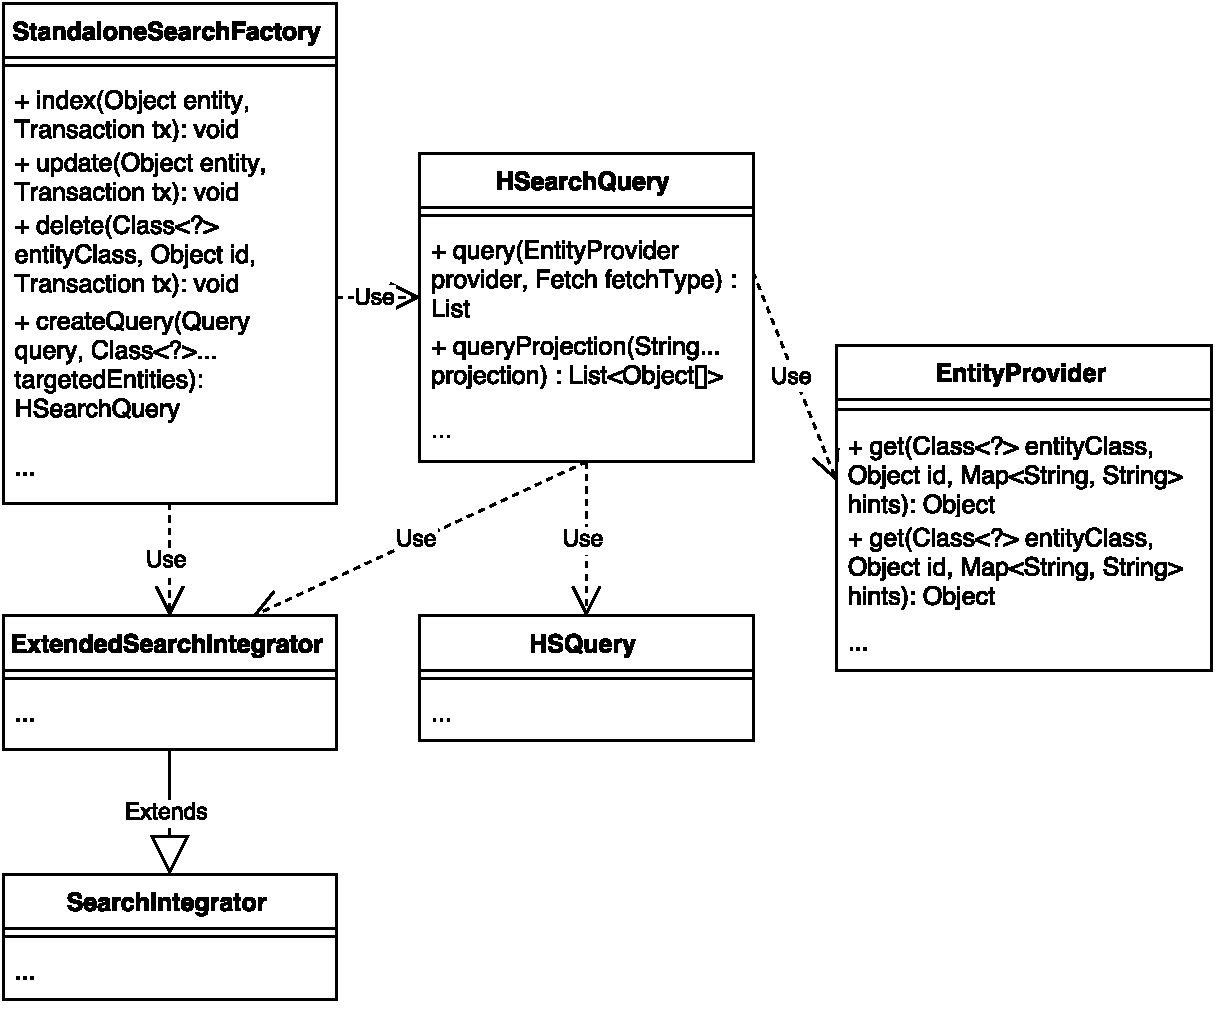
\includegraphics[scale=0.6]{images/standalone_min_architecture.pdf}
	\caption{Rough architecture of the standalone version (important parts)}
	\label{standalone_min_architecture}
\end{figure}

\pagebreak

\subsubsection{Startup}

The startup process of the standalone version doesn't differ much from manually using the engine in terms of configuration as we still have to use the SearchConfiguration interface. The only difference is how we build the StandaloneSearchFactory. This is done with a \textbf{StandaloneSearchFactoryFactory}, so the code using it doesn't have to handle the creation of the actual implementation object.
\\
\lstset{language=java}
\lstset{moredelim=[is][\bfseries]{[*}{*]}}
\begin{lstlisting}[frame=htrbl, caption={Starting up the standalone version}, label={lst:using_standalone.java}]
List<Class<?>> indexClasses = Arrays.asList(Book.class, Author.class);

//we still have to build the SearchConfiguration object
SearchConfiguration searchConfiguration = 
		new StandaloneSearchConfiguration();
indexClasses.forEach( searchConfiguration::addClass );

//the builder pattern from before is abstracted in the following lines
StandaloneSearchFactory searchFactory = 
		StandaloneSearchFactoryFactory.
				createSearchFactory(
					searchConfiguration,
					indexClasses
				);
				
//use the searchfactory ...

//close it
searchFactory.close();
\end{lstlisting}

\pagebreak

\subsubsection{Index manipulation}

With our standalone version, basic index control becomes more streamlined as we don't have to work with the SearchIntegrator's Worker pattern anymore as it was described in chapter \ref{index_manipulation_integrator}:
\\
\lstset{language=java}
\begin{lstlisting}[frame=htrbl, caption={Indexing an object with the standalone version}, label={lst:indexing_object_native.java}]objects
Book book = ...;
Transaction tx = new Transaction();
searchFactory.index(book, tx);
tx.commit();
\end{lstlisting}

\lstset{language=java}
\begin{lstlisting}[frame=htrbl, caption={Updating an object with the standalone version}, label={lst:updating_object_native.java}]
Book book = ...;
Transaction tx = new Transaction();
searchFactory.update(book, tx);
tx.commit();
\end{lstlisting}

\lstset{language=java}
\begin{lstlisting}[frame=htrbl, caption={Deleting an object by id with the standalone version}, label={lst:deleting_object_native.java}]
Transaction tx = new Transaction();
String isbn = ...;
searchFactory.delete(Book.class, isbn, tx);
tx.commit();
\end{lstlisting}

\pagebreak

\subsubsection{Queries} \label{querying_standalone}
The biggest change in the standalone version is probably how the index is queried. We don't have to work with EntityInfos anymore as we introduced the \textbf{EntityProvider} interface. This interface hosts one method that is to be used for batch fetching (Fetch.BATCH) and one for single fetching (Fetch.FIND\_BY\_ID).
\\\\
A good default implementation delegating the database access to a JPA EntityManager is our \textbf{BasicEntityProvider} (listing \ref{lst:BasicEntityProvider.java} in the appendix). Besides taking an EntityManager in its constructor, it also needs a Map<Class<?>, String> containing the id properties of the entities. While we leave the construction of this map out in the following listing \ref{lst:querying_standalone123.java} for the sake of simplicity, the code for this can be found in listing \ref{lst:idProperties.java} in the appendix. After its creation, this map can then be stored in a central place and reused.
\\
\lstset{language=java}
\begin{lstlisting}[frame=htrbl, caption={Querying the index with the standalone version}, label={lst:querying_standalone123.java}]
StandaloneSearchFactory searchFactory = ...;

EntityManager em = ...;
Map<Class<?>, String> idProperties = ...;

EntityProvider entityProvider = new BasicEntityProvider(em, idProperties);

List<Book> books = searchFactory
			.createQuery(searchFactory.buildQueryBuilder()
				.forEntity(Book.class)
				.get()
				.keyword()
				.onField("title")
				.matching("searchString")
				.createQuery(), Book.class
			).query(
				entityProvider,
				Fetch.BATCH
			);
\end{lstlisting}

\pagebreak
~
\pagebreak

\section{JPA integration of the standalone version} \label{integration_jpa}

\begin{figure}[ht]
	\centering
	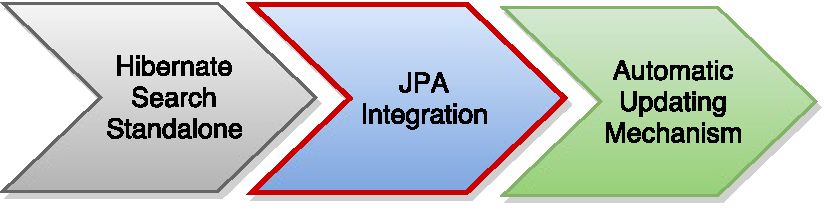
\includegraphics[scale=0.75]{images/timeline_genericjpa_second.pdf}
	\label{project_timeline_second}
\end{figure}
\noindent
After simplifying the access to Hibernate Search's engine we will work out an integration with JPA interfaces next. Since we started with the premise of not wanting to "reinvent the wheel" by writing everything from scratch (as described in \ref{reinvent_the_wheel}), we will try to build an integration as similar to the JPA interfaces of Hibernate Search ORM as possible.
\\\\
Before we can go into detail about how we build our integration, we have to discuss the general architecture first. We will go over how the Hibernate Search ORM integration with JPA interfaces behaves from a user's point of view and then take a look at what has to be changed in order to be compatible with any JPA implementor.

\pagebreak

\subsection{Architecture of Hibernate Search ORM}

Hibernate Search ORM integrates with the JPA API by extending the interfaces  javax.persistence.EntityManager and javax.persistence.Query and adds new functionality to the fulltext search versions of these interfaces: \textbf{FullTextEntityManager} and \textbf{FullTextQuery}. The following figure shows a rough overview of this. Note that this contains only the methods relevant for the following sections.
\\
\begin{figure}[ht]
	\centering
	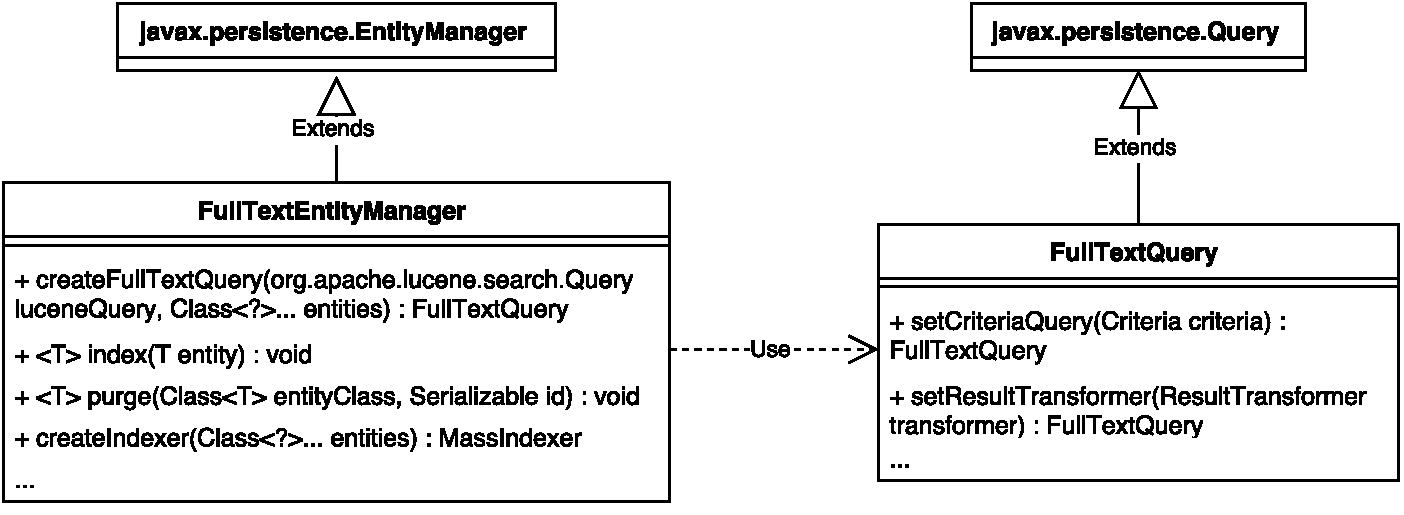
\includegraphics[scale=0.6]{images/hibernate_search_jpa_integration_original.pdf}
	\caption{The main JPA interfaces of Hibernate Search ORM}
	\label{hibernate_search_jpa_integration_original}
\end{figure}

\pagebreak

\subsubsection{Startup} \label{startup_original}
As Hibernate Search ORM is tightly coupled with Hibernate ORM it is automatically started if found on the classpath and the persistence.xml contains the following:
\\
\lstset{language=java, breaklines=true}
\begin{lstlisting}[frame=htrbl, caption={Additions to persistence.xml with Hibernate Search ORM}, label={lst:hibernate_search_persistence.xml}]
...
<property name="hibernate.search.default.directory_provider" value="filesystem"/>
<property name="hibernate.search.default.indexBase" value="/path/to/indexes"/>
...
\end{lstlisting}
\noindent
This means that there exists no real code entry point as Hibernate Search is fully integrated into the Hibernate ORM/OGM lifecycle. FullTextEntityManagers can therefore be obtained with:
\\
\lstset{language=java}
\begin{lstlisting}[frame=htrbl, caption={Obtaining a FullTextEntityManager with Hibernate Search ORM}, label={lst:indexing_object_hsearch_orm_jpa.java}]
EntityManager em = ...;
FullTextEntityManager fem = Search.getFullTextEntityManager(em);
\end{lstlisting}
All of FullTextEntityManager's operations are controlled by the same transactions the original Hibernate EntityManager is using. This is the reason we will not have any search transaction related code in the following paragraphs.

\pagebreak

\subsubsection{Index manipulation}
The index operations are all straightforward and similar to what we designed our standalone version in chapter \ref{standalone_hibernate_search} to work like apart from minor naming differences. 
\\\\
Hibernate Search ORM doesn't differentiate between indexing and updating.
\\
\lstset{language=java}
\begin{lstlisting}[frame=htrbl, caption={Indexing/Updating an object with Hibernate Search ORM}, label={lst:indexing_object_hsearch_orm_jpa.java}]
FullTextEntityManager fem = ...;
Book book = ...;
fem.index(book);
\end{lstlisting}
\noindent
Deleting objects from the index is called purging. This is probably due to not wanting to confuse it with JPA's delete(...).
\\
\lstset{language=java}
\begin{lstlisting}[frame=htrbl, caption={Deleting an object by id with Hibernate Search ORM}, label={lst:deleting_object_hsearch_orm_jpa.java}]
FullTextEntityManager fem = ...;
String isbn = ...;
fem.purge(Book.class, isbn);
\end{lstlisting}

\pagebreak

\subsubsection{Queries} \label{hsearch_orm_querying}
Hibernate Search ORM integrates even better with JPA for queries than our standalone version as the FullTextQuery interface extends the JPA Query interface and uses getResultList() to return its results:
\\
\lstset{language=java}
\begin{lstlisting}[frame=htrbl, caption={Querying with Hibernate Search ORM}, label={lst:querying_hsearch_orm.java_1}]
EntityManager em = ...;
FullTextEntityManager fem = Search.getFullTextEntityManager(em);

FullTextQuery fullTextQuery = fem.createFullTextQuery(
	fem.getSearchFactory().buildQueryBuilder()
		.forEntity( Book.class )
		.get()
		.keyword()
		.onField( "title" )
		.matching( "searchString" )
		.createQuery(), 
	Book.class);
	
List<Book> books = (List<Book>) fullTextQuery.getResultList();
\end{lstlisting}

\pagebreak

\subsubsection{Index rebuilds}
A noteworthy feature of Hibernate Search is its MassIndexer. It can be used whenever the way the entities are indexed is changed (e.g. in the @Field annotations). It uses multiple threads working in parallel to scroll results from the database and then indexes these efficiently. This is by far faster than the naive approach working in only one thread. It also incorporates a lot of internal improvements a normal developer wouldn't have access to as the specifics are hidden in the implementation packages of Hibernate Search which are not intended to be used outside of its own code.
\\\\
A full index rebuild for our Book entity would look like this:
\\
\lstset{language=java}
\begin{lstlisting}[frame=htrbl, caption={MassIndexer usage with Hibernate Search ORM}, label={lst:massindexing_hsearch_orm.java}]
EntityManager em = ...;
FullTextEntityManager fem = Search.getFullTextEntityManager(em);

fem.createIndexer( Book.class )
	.batchSizeToLoadObjects( 25 )
	.threadsToLoadObjects( 12 )
	.idFetchSize( 150 )
	.transactionTimeout( 1800 )
	.startAndWait();
\end{lstlisting}
\noindent
"This will rebuild the index of all [Book] instances (and subtypes), and will create 12 parallel threads to load the User instances using batches of 25 objects per query; these same 12 threads will also need to process indexed embedded relations and custom FieldBridges or ClassBridges, to finally output a Lucene document."\footnote{Hibernate Search documentation (MassIndexer, v5.4), see~\cite{hibernate_search_doc_massindexer}}

\pagebreak

\subsection{Architecture of the generic version}

As good as Hibernate Search ORM's API integration with JPA's EntityManager and Query interface is, its additional interfaces still contain some Hibernate ORM related features and logic that a generic version (we call it Hibernate Search GenericJPA) can not support and therefore have to be changed, emulated or removed altogether.
\\
\begin{figure}[ht]
	\centering
	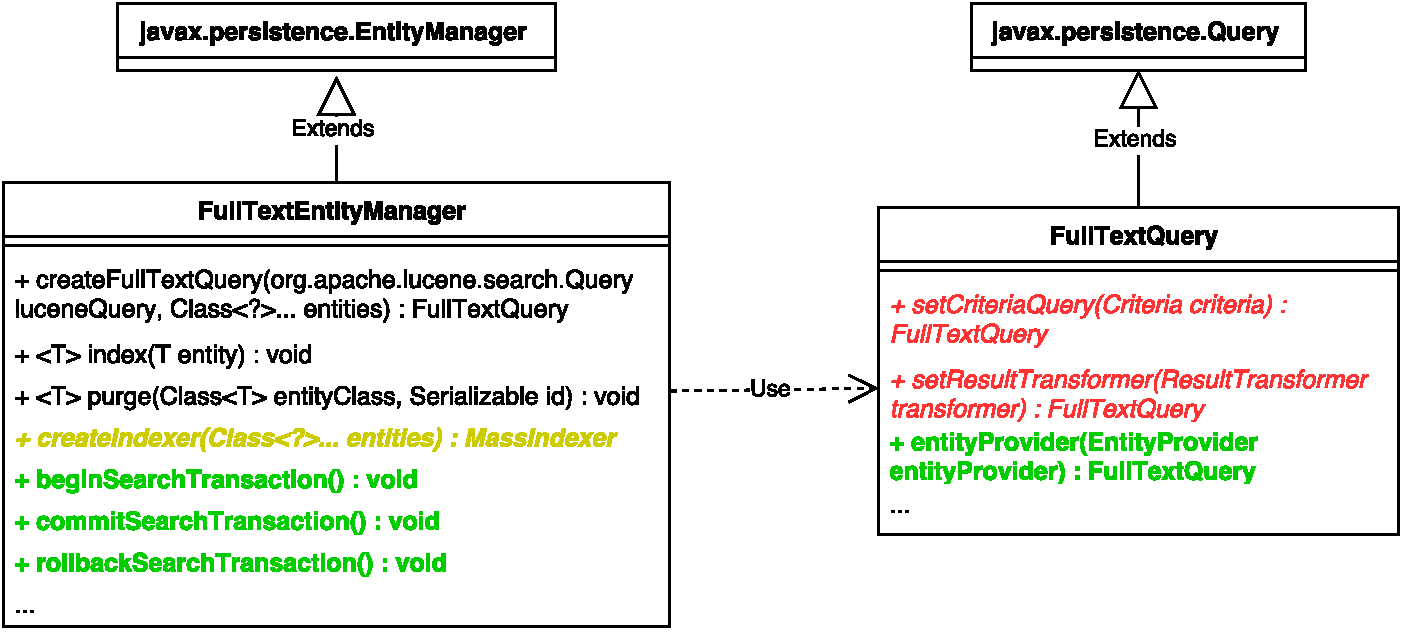
\includegraphics[scale=0.6]{images/hibernate_search_jpa_integration_with_differences.pdf}
	\caption{Required fixes for a generic version}
	\label{hibernate_search_jpa_integration_with_differences}
\end{figure}
\\
In the figure \ref{hibernate_search_jpa_integration_with_differences} above, we have marked all the methods requiring to be fixed in the FullTextEntityManager and FullTextQuery interfaces:
\begin{itemize}
	\item green: new methods
	\item red: methods that can't be supported
	\item olive: methods that can be supported if changed
\end{itemize}
\noindent
Besides these, some other aspects need changes as well. We will describe the reasoning behind all of the needed changes \& additions in the following paragraphs.

\pagebreak

\subsubsection{Startup}

In our generic version we can't tightly integrate with the EntityManagerFactory of the JPA provider. This is the reason we introduce a separate interface called \textbf{JPASearchFactoryController}:
\\
\begin{figure}[ht]
	\centering
	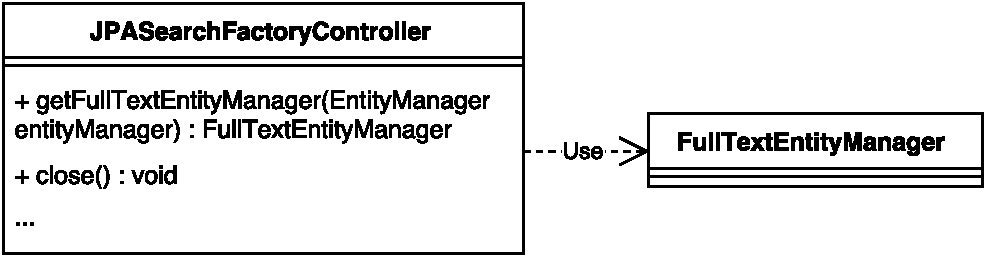
\includegraphics[scale=0.6]{images/JPASearchFactoryController.pdf}
	\caption{JPASearchFactoryController}
	\label{jpa_searchfactory_controller}
\end{figure}

\noindent
Having this separate interface means that the lifecycle of the generic version has to be controlled separately contrary to the standard Hibernate Search which is integrated with Hibernate ORM's lifecycle as described in chapter \ref{startup_original}.
\\\\
Unlike the static way a FullTextEntityManager is obtained in Hibernate Search ORM via the Search class, in our generic version, we obtain it with the \textbf{getFullTextEntityManager(EntityManager entityManager)} method (the Search class in Hibernate Search ORM only works because of the tight coupling of ORM and Search). This means that an instance of the JPASearchFactoryController has to be available at all times when access to the index is required.
\\\\
Using a non-static approach here has one benefit, though: we can pass null to this method and get a search only FullTextEntityManager that can be used to work on the index when no database access is needed. This is particularly useful if POJOs have to be indexed which are not associated with JPA (see table \ref{table:config_properties_jpasearchfactorycontroller}, property "hibernate.search.additionalIndexedTypes").

\pagebreak

\noindent
We start the fulltext search engine with our bootstrapping class \textbf{Setup} like this:
\\
\lstset{language=java}
\begin{lstlisting}[frame=htrbl, caption={MassIndexer usage with Hibernate Search ORM}, label={lst:massindexing_hsearch_orm.java}]
//In Hibernate Search ORM, the fulltext engine would be started 
//together with the EntityManagerFactory.
//In GenericJPA we can't do that.
EntityManagerFactory emf = ...;

EntityManager em = ...;

Properties properties = new Properties();

properties.setProperty(
	"hibernate.search.searchfactory.type", 
	"manual-updates"
);

//In GenericJPA this starts the fulltext engine to 
//which a reference is returned by this method call
JPASearchFactoryController searchFactoryController =
	Setup.createSearchFactoryController( emf, properties );

//FullTextEntityManagers are not obtained with the Search class
FullTextEntityManager fem = 
	searchFactoryController.getFullTextEntityManager(em);

//use it...

searchFactoryController.close();
\end{lstlisting}
\noindent
For this example we are using "manual-updates", as we haven't discussed how the index is kept up-to-date. After we worked that out, "manual-updates" will just be a fallback setting for developers not wanting to have the index automatically updated.  Also note that there are many more properties that can be set and that vanilla Hibernate Search settings are passed this way as well. A complete list of the available GenericJPA configuration properties can be found in table \ref{table:config_properties_jpasearchfactorycontroller} in the appendix.

\pagebreak

\subsubsection{Index manipulation} \label{using_hsearch_genericjpa_index}

In Hibernate Search ORM, all manual index manipulations are synchronized with the EntityManager transaction lifecycle (index changes underly the JPA transaction system). In our generic approach we cannot do this as JPA doesn't have an extension point for this kind of usage. This is the reason we introduce the \textbf{[begin/commit/rollback]SearchTransaction()} methods in FullTextEntityManager. These have to be used to control the transaction lifecycle of all the index manipulation methods:
\\
\lstset{language=java}
\begin{lstlisting}[frame=htrbl, caption={Index control with Hibernate Search GenericJPA}, label={lst:index_control_hibernatesearchgenericjpa}]
EntityManager em = ...;
JPASearchFactoryController searchFactoryController = ...;

FullTextEntityManager fem = 
	searchFactoryController.getFullTextEntityManager(em);

fem.beginSearchTransaction();
try {
	//index or purge here
	fem.commitSearchTransaction();
} catch(Exception e) {
	fem.rollbackSearchTransaction();
	throw e;
}
\end{lstlisting}
\noindent
Because manual index changes are not needed frequently in normal applications, we don't restrict the usage of GenericJPA in application servers by a lot compared to the original Hibernate Search ORM by introducing our own search transaction management methods. In general, Hibernate Search transactions can not be compared with real RDBMS transactions anyways as it is allowed to write changes to the index without commiting with flushToIndexes(). Changes applied in this manner can not be reverted by a rollback.

\pagebreak
\noindent
One additional problem with supporting indexing generic JPA entities is that some JPA providers don't return objects of the original entity class. For example, EclipseLink returns an object of an anonymous subclass of the original in which it hides away some utility logic needed for lazy loading.
\\\\
This is problematic because the engine needs to know which class to get the index description metamodel from. Therefore we have to implement logic to feed the right entity class into the engine via user input for Hibernate Search GenericJPA. Entity classes have to be marked with \textbf{@InIndex} on the type level so we can start from any object's class and then go up in the class hierarchy until we find one that is annotated with this annotation. If no @InIndex is found, we use the actual class of the entity object we are about to index as a best effort (this is the behaviour Hibernate Search ORM has). This algorithm is described in Java code in the next listing \ref{lst:algo_subclasssupport}:
\\
\lstset{language=java}
\begin{lstlisting}[frame=htrbl, caption={Algorithm to determine the actual indexed type}, label={lst:algo_subclasssupport}]
//get the first class in the hierarchy
Class<T> clazz = (Class<T>) entity.getClass();

//check if the original class has @InIndex present
//if yes, we don't have to go higher up in the class hierarchy
if ( !clazz.isAnnotationPresent( InIndex.class ) ) {

	//go up in the class hierarchy until either a @InIndex is found
	//or there is no superclass anymore.
	while ( (clazz = (Class<T>) clazz.getSuperclass()) != null ) {
		if ( clazz.isAnnotationPresent( InIndex.class ) ) {
			break;
		}
	}
	
}

//if we have found a class annotated with @InIndex
//we return it here
if ( clazz != null ) {
	return clazz;
}

//no @InIndex found, try the entities direct class
//as a best effort
return entity.getClass();
\end{lstlisting}

\pagebreak
\noindent
Note that every entity that is part of the index has to be annotated with @InIndex, even the ones that are just embedded. With this in mind our entities Book and Author now look like this:
\\
\lstset{language=java}
\lstset{moredelim=[is][\bfseries]{[*}{*]}}
\begin{lstlisting}[frame=htrbl, caption={Book.java with @InIndex}, label={lst:book.java_2}]
@Entity
[*@InIndex*]
@Table(name = "Book")
@Indexed
public class Book {
	
	//rest is unchanged

}
\end{lstlisting}

\lstset{language=java}
\lstset{moredelim=[is][\bfseries]{[*}{*]}}
\begin{lstlisting}[frame=htrbl, caption={Author.java with @InIndex}, label={lst:author.java_2}]
@Entity
[*@InIndex*]
@Table(name = "Author")
public class Author {
	
	//rest is unchanged
	
}
\end{lstlisting}
\noindent
A similar behaviour supporting the subclassing of entities can be achieved with JPA's @Entity  replacing the @InIndex annotation as these annotations can be found on the first real entity class in the hierarchy as well. We didn't choose this approach because by using @InIndex we support indexing of non-JPA entities as well. A hybrid approach checking for both annotations might be possible, but using only @InIndex is sufficient for now.

\pagebreak

\subsubsection{Queries}
While we didn't mention this in chapter \ref{hsearch_orm_querying}, Hibernate Search ORM supports modifying the resulting objects of a query with these two methods on \textbf{FullTextQuery}:

\begin{itemize}
	\item \textbf{setCriteriaQuery(Criteria criteria)}:
		This method lets the user define a custom Hibernate Criteria query (no JPA criteria query) that has to be used to retrieve the results from the database. This can be used to make sure all necessary data is loaded after it is returned by getResultList(). These custom queries are  used in cases where no session is available anymore when the data is finally used: If the data is requested, an error would occur.
	\item \textbf{setResultTransformer(ResultTransformer resultTransformer)}:
		A ResultTransformer can be used to transform the results (useful for projections) into POJOs (Plain Old Java Object).
\end{itemize}
\noindent
There is a problem with these two methods, though. They are using the Hibernate ORM API to accomplish their behaviour, and therefore we cannot support the methods on our generic version of the interface.
\\\\
By adding a new method \textbf{entityProvider(EntityProvider entityProvider)} with the same EntityProvider interface as in chapter \ref{querying_standalone} to the method, we can at least support custom queries.
\\\\
As the main use case scenario for the ResultTransformer is probably just the transformation from a projection of the queried documents to a POJO, we just completely remove this feature. In the future, we can add such a feature back to the generic version, if needed. But as this method cannot be kept as-is anyways, Hibernate Search ORM developers wanting to use Hibernate Search GenericJPA that use this feature have to change some of their code either way.
\\\\
Besides these changes, the interface behaves the exact same as described in \ref{hsearch_orm_querying}.

\pagebreak

\subsubsection{Index rebuilds}

The MassIndexer utility is a really important feature of Hibernate Search ORM. As it uses Hibernate ORM logic under the hood (and in its interface), we have to write our own version of it. We don't build an API compatible version for Hibernate Search GenericJPA as a MassIndexer is generally not used in many places in the code anyways. Additionally this way we can give different configuration properties for better performance as our implementation differs in some details.
\\\\
The basic ideas are the same though: Each entity type has its ids scrolled from the database by one thread (there can be multiple threads doing this, but for other entities). Then, a configurable amount of indexing threads handles these ids batch by batch in a Hibernate Search index-writing backend optimized for this task (this is part of Hibernate Search's engine is therefore reused).
\\\\
In Hibernate Search GenericJPA our Book entities are massindexed like this:
\\
\lstset{language=java}
\begin{lstlisting}[frame=htrbl, caption={MassIndexer usage with Hibernate Search ORM}, label={lst:massindexing_hsearch_orm.java}]
EntityManager em = ...;
FullTextEntityManager fem = Search.getFullTextEntityManager(em);

fem.createIndexer( Book.class )
	.batchSizeToLoadObjects( 25 )
	.threadsToLoadObjects( 12 )
	.batchSizeToLoadIds( 150 )
	.idProducerTransactionTimeout( 1800 )
	.startAndWait();
\end{lstlisting}

\pagebreak

% !TeX spellcheck = en_GB

\section{Automatic index updating} \label{automatic_indexing_chapter}

\begin{figure}[ht]
	\centering
	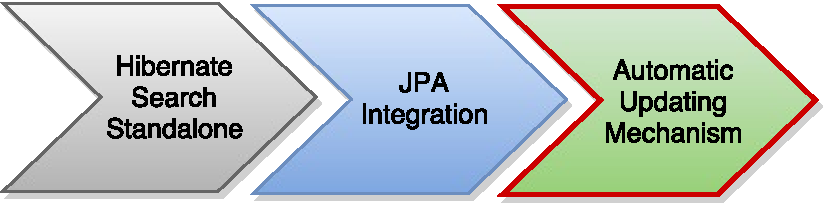
\includegraphics[scale=0.75]{images/timeline_genericjpa_third.pdf}
	\label{project_timeline_third}
\end{figure}
\noindent
As already stated in chapter \ref{automatic_indexing_problematic_intro}, the automatic index updating feature is required for a reasonable Hibernate Search GenericJPA. As this is arguably the most complicated feature for GenericJPA, we will go into detail about how we are achieving it next. We will start by giving a description of the different implementations available and then decide which ones to use. We are however not showing the complete internal code architecture - like in chapters \ref{standalone_chapter} and \ref{integration_jpa} - in favour of explaining in detail how the general ideas work. After that, we will also give a short overview of the pros and cons of the chosen approaches. 

\pagebreak

\subsection{Description of different implementations} \label{description_of_different_implementations}

There are several approaches to building an automatic index updating feature. While they are all different in the specifics, they can generally be separated into two categories: \textbf{synchronous} and \textbf{asynchronous}. Synchronous in this context means that the index is updated as soon as the newly changed data is persisted in the database without any real delay while in an asynchronous updating mechanism an arbitrary amount of time passes before the index is updated. While synchronous approaches are needed in some rare cases, fulltext search generally doesn't require a 100\% up-to-date index at every point in time  as a search index generally is not the source of truth in an application (only the database contains the "truth").
\\\\
We will now work out a solution for both the synchronous and asynchronous case, while the asynchronous version will serve as a backup whenever the synchronous mechanism is not applicable.

\pagebreak

\subsubsection{Synchronous approach}

For the synchronous approach we have two candidates: A system based on JPA callback events and another one that uses the native APIs of JPA providers. We start with the JPA callbacks and then go onto the native APIs.

\paragraph{JPA events}

As we are trying to work with as little vendor specific APIs, JPA's callback events look like a suitable candidate for listening to changes in entities.
\\\\
To listen for the JPA events we have two options: annotate the entities with callback methods or create a separate listener class. We will only take a look at the listener class since we don't want to have unnecessary methods in a possible user's entities. This listener class doesn't have to implement an interface, but must have methods annotated with special annotations. The relevant ones are @PostPersist, @PostUpdate, @PostDelete (there are "pre-versions" available as well, but we focus on the post methods as they are more useful). What each specific annotation stands for is quite self-explanatory.
\\\\
A listener class generally looks like this:
\\
\lstset{language=java}
\lstset{moredelim=[is][\bfseries]{[*}{*]}}
\begin{lstlisting}[frame=htrbl, caption={Example JPA entity listener}, label={lst:jpa_entity_listener.java}]
public class EntityListener {

	@PostPersist
	public void persist(Object entity) {
		//handle the event
	}
	
	@PostUpdate
	public void update(Object entity) {
		//handle the event
	}
	
	@PostDelete
	public void delete(Object entity) {
		//handle the event
	}

}
\end{lstlisting}

\pagebreak

\noindent
These EntityListeners are generally applied with an annotation on the entity:
\\
\lstset{language=java}
\lstset{moredelim=[is][\bfseries]{[*}{*]}}
\begin{lstlisting}[frame=htrbl, caption={Using a JPA entity listener}, label={lst:using_jpa_entitylisteners.java}]
[*@EntityListeners( { EntityListener.class } )*]
public class Book {

	//...

}
\end{lstlisting}
\noindent
As the JPA provider creates the EntityListeners automatically, we have no access to them without injecting a reference to them in a static way. While this might cause some Classloader problems, it should be fine in most cases.
\\
\lstset{language=java}
\lstset{moredelim=[is][\bfseries]{[*}{*]}}
\begin{lstlisting}[frame=htrbl, caption={Injecting the EntityListener}, label={lst:jpa_entity_listener.java}]
public class EntityListener {

	public EntityListener() {
		// inject it somewhere
		// so we can access it in a static way
		EntityListenerRegistry.inject(this);
	}

	//...

}
\end{lstlisting}

\pagebreak

\noindent
Even though these listeners seem to be the perfect fit as they would enable us to fully integrate only with JPA interfaces, they have two big issues as we find out after investigating further.
\\\\
Firstly, not all JPA providers seem to handle these events similarly: For example Hibernate ORM doesn't propagate events from collection tables to the owning entity, while EclipseLink does (EclipseLink's behaviour would be needed from all providers).
\\\\
Secondly, we find out that the events are triggered on flush instead of commit as can be seen in listing \ref{lst:flush_event.java}. This is an issue if the changed data is not actually commited:
\\

\lstset{language=java}
\lstset{moredelim=[is][\bfseries]{[*}{*]}}
\begin{lstlisting}[frame=htrbl, caption={Event triggering on flush}, label={lst:flush_event.java}]
EntityManager em = ...;

em.getTransaction().begin();

Book book = em.find( Book.class, "someIsbn" );
book.setTitle( "someNewTitle" );

// flushes, so we retrieve the Book with the changes from above
// => event is triggered
List<Book> allBooks = 
	em.createQuery( "SELECT b FROM Book b" ).getResultList();

// we have no way to get this event to revert the wrong index change
em.getTransaction().rollback();
\end{lstlisting}

\noindent
While it \textbf{might} be possible to somehow fix the flush issue, the general bad support from JPA providers like Hibernate ORM renders this approach unusable until the JPA providers work the same way regarding the event propagation to some reasonable extent.

\pagebreak

\paragraph{Native integration with JPA providers}

Almost every JPA provider has its own internal event system that is useful for cache invalidation and other tasks. These combined with hooks into the transaction management allow us to build a proper index updating system that works with transactions in mind (big improvement compared to the flush() issues of plain JPA).
\\\\
JPA providers generally have callbacks similar to those of the JPA events (no knowledge about database specifics is needed, Java types are used), but also provide additional information about the database session that caused the changes.
\\\\
By definition, these kind of integrations are not portable between JPA providers and require us to write different systems for all the JPA providers. But as the landscape for popular JPA providers probably only consists of Hibernate ORM, EclipseLink and OpenJPA, we can implement listeners for these and the others will have to rely on the asynchronous backup approach (as of the time of writing this, we have only implemented integrations for Hibernate ORM and EclipseLink).
\\\\
As this seems to be the only reasonable solution for a synchronous update system, we are using it for Hibernate Search GenericJPA even though it is no real native solution because of the JPA implementation dependent code.
\\\\
\textit{Note: we don't describe how these event systems are built in particular as they differ a lot in their APIs, but generally these are straightforward to use and describing the implementations would be unspectacular.}

\pagebreak

\subsubsection{Asynchronous approach}\label{async_approach}
In contrary to the synchronous approach where we described two different versions, for the asynchronous version we only have one feasible solution available: a trigger based system.
\\\\
Paul DuBois writes in MySQL - Developer's Library:
\begin{quote}
	A Trigger is a stored program that is associated with a particular table and is defined to activate for INSERT, DELETE or UPDATE statements for that table. A trigger can be set to activate either before or after each row processed by the statement. The trigger definition includes a statement that executes when the trigger activates.
	\\\\
	~[...]~
	\\\\
	A trigger can examine the current contents of a row before it is deleted or updated. This capability can be exploited to perform logging of changes [...].
	\footnote{MySQL - Developer's Library, see~\cite{mysql_developers_lib}}
\end{quote}
\noindent
While the quote above is meant to be for MySQL databases, many other RDBMSs support at least triggers on the three crucial events for event-listening: INSERT (CREATE), UPDATE, DELETE, just like MySQL \footnote{CREATE TRIGGER in PostgreSQL, see~\cite{postgres_triggers}} \footnote{Triggers in HSQLDB, see~\cite{hsqldb_triggers}} \footnote{Triggers in Firebird, see~\cite{firebird_triggers}}.
\\\\
In order to have triggers being useful for updating our Hibernate Search index, we have to get info about the events from the database back into our Java application. Since we cannot necessarily call Java code from our database (with the exception of some enterprise and in-memory databases), we have to write data about changes into auxiliary tables and then poll these regularly.
\\\\
One benefit of this approach is that by using polling from the tables and the fact that triggers are executed in the same transaction as the original changing query, we don't have to manually hook into transactions or deal with data that has not been committed, yet, in general. If we do things right, we can even improve indexing performance by this: We can query for the latest event for each entity only, so we don't use up an unnecessary amount of CPU-time, but still keep the index up-to-date.

\pagebreak

\paragraph{Trigger architecture}

Triggers are generally created on tables. Since we want to use them for event-listening, we have to cover every table of the domain model that contains data indexed/stored in the index. This also includes all of the mapping tables between entities and all other secondary tables.
\\\\
The following figure \ref{triggers_schema} shows the trigger architecture needed for our Author and Book example. Note that we are using triggers that execute before changes are persisted.
\\
\begin{figure}[ht]
	\centering
	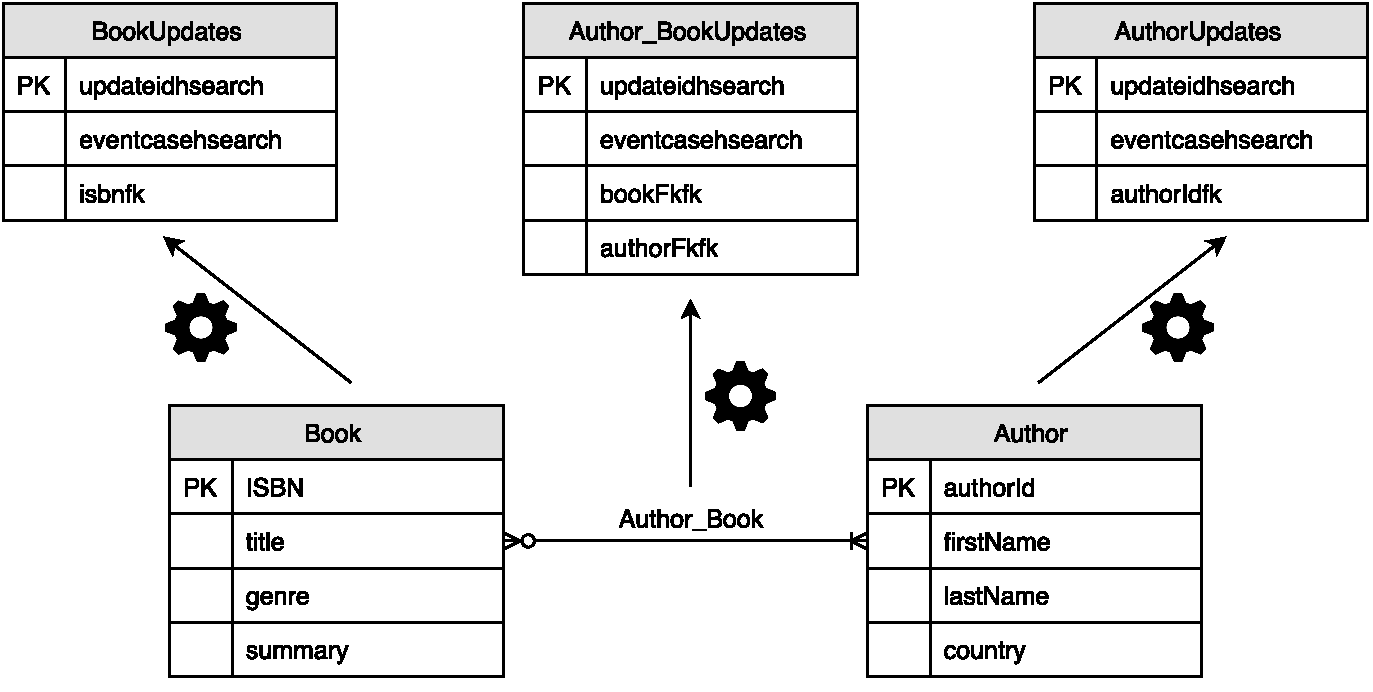
\includegraphics[scale=0.6]{images/Triggers_Schema.pdf}
	\caption{Triggers for the example project}
	\label{triggers_schema}
\end{figure}
\\
\noindent
All three tables Author, Book and Author\_Book have three triggers registered on them (one for each event type). These triggers then fill up the update tables AuthorUpdates, BookUpdates and Author\_BookUpdates (these names are just for demonstrative purposes) with info about occurring events. We can see that these update tables host at least three things:

\begin{enumerate}
	\item \textbf{updateid primary key:} Update events have to be sortable by the order they occured. All update tables share the same sequence of primary keys so that no key appears twice in all of these tables.
	\item \textbf{eventcase column:} This column contains a identifier for the cases INSERT, DELETE or UPDATE.
	\item \textbf{pseudo foreign key(s):} The relevant primary keys of the entities involved in the tables have to be stored in the Update tables as well. Note that they are not marked as real foreign keys as a DELETE event wouldn't work as we can't have a reference to a non existent entity.
\end{enumerate}

\pagebreak

\paragraph{Table creation} \label{creating_the_tables}

Since the creation of these tables requires a lot of work to be done, we have to automate it as well as possible. We do this by requiring additional \textbf{@UpdateInfo} annotations on the entities to map the required information for the update tables and then generating them out of it.
\\\\
These annotations contain at least the original table's name (UpdateInfo\#tableName) and the names \& types (IdColumn\#column \& IdColumn\#columnType) of the entity key columns. The name of the update table and the columns in it are then generally derived automatically from that. 
\\\\
A similar behaviour might be possible by using the JPA mapping annotations to read the original schema and then deduce the needed update schema from that. We don't use this approach nonetheless, because the task of parsing these annotations correctly would be prone to errors due to the amount of different annotations (@Basic, @Column, @IdClass, @EmbeddedCollection, @OneToOne, @ManyToOne, @OneToMany, @ManyToMany, ...). In some cases these annotations aren't even required for JPA to work, which makes it even more complicated. This makes the approach less streamlined than using the extra @UpdateInfo annotations.

\pagebreak
\noindent
The following listings show the @UpdateInfo annotation in use:
\\
\lstset{language=java}
\lstset{moredelim=[is][\bfseries]{[*}{*]}}
\begin{lstlisting}[frame=htrbl, caption={Book.java with Hibernate Search annotations}, label={lst:book.java_3}]
@Entity
@InIndex
@Table(name = "Book")
@Indexed
[*@UpdateInfo(
	tableName = "Book", 
	idInfos = @IdInfo(
		columns = @IdColumn(
			column = "isbn", 
			columnType = ColumnType.STRING
		)
	)
)*]
public class Book {

	// ... unchanged. 
	
	// mapping table events handled on Author side
	
	// getters & setters ...
}
\end{lstlisting}

\pagebreak

\lstset{language=java}
\lstset{moredelim=[is][\bfseries]{[*}{*]}}
\begin{lstlisting}[frame=htrbl, caption={Author.java with Hibernate Search annotations}, label={lst:author.java_3}]
@Entity
@InIndex
@Table(name = "Author")
[*@UpdateInfo(
	tableName = "Author", 
	idInfos = @IdInfo(
		columns = @IdColumn(
			column = "authorId", 
			columnType = ColumnType.LONG
		)
	)
)*]
public class Author {
	
	// ... unchanged.
	
	[*@UpdateInfo(tableName = "Author_Book", 
		idInfos = {
		@IdInfo(entity = Author.class, 
			columns = @IdColumn(
				column = "authorFk",
				columnType = ColumnType.LONG
			)
		),
		@IdInfo(entity = Book.class,
			columns = @IdColumn(
				column = "bookFk",
				columnType = ColumnType.STRING
			)
		)
	})*]
	private Set<Book> books;
	
	//getters & setters ...
}
\end{lstlisting}
\noindent
\textit{Note: The update tables are NOT JPA entities, so we have to work with native SQL in the backend}.
\\\\
\noindent
If the developer needs different names for the update tables and their columns (e.g. if there already exists a table with the same name), it is possible to manually set these. They can be found on the same level in the annotations as the corresponding info for the original table is set.

\pagebreak

\noindent
Options for multivalued keys and custom column types are also available as by default only singular valued keys of the column types corresponding to Java's Integer, Long and String are supported. While we don't go into detail how these expert features are used, information about how to use them can be found in the JavaDoc of the annotations.
\\\\
Since database triggers and tables are not created the same on every RDBMS, we build an abstraction to get the necessary SQL code. This is done with the \textbf{TriggerSQLStringSource} interface. Its implementations return the specific SQL strings working on the corresponding RDBMS. As of this writing we have implementations for MySQL, PostgreSQL and HSQDLB. See the property "hibernate.search.trigger.source" in table \ref{table:config_properties_jpasearchfactorycontroller} in the appendix for information about how to set the correct one for each database.
\\\\
This table also contains a property called "hibernate.search.trigger.createstrategy" that controls whether and how the triggers and tables are generated at all. If automatic trigger creation is disabled, the user still has to provide the information about the update tables that should be used for updating with the annotations as described above.

\pagebreak

\paragraph{Event retrieval}
Now that we know how the events are stored in the update tables, we will describe an efficient way to query the database for these entries.
\\\\
We only need the latest event for each entity (or combination of entities for mapping tables). The following SQL query shown in listing \ref{lst:querying_updates.sql} is doing this for the table author\_bookupdates with standard SQL that should be working on every RDBMS:
\\
\lstset{language=sql}
\lstset{moredelim=[is][\bfseries]{[*}{*]}}
\begin{lstlisting}[frame=htrbl, caption={Querying for updates (Author\_Book)},
label={lst:querying_updates.sql}]
SELECT t1.updateidhsearch, t1.authorFkfk, t1.bookFkfk
FROM author_bookupdates t1
INNER JOIN
(
	/* select the most recent update */
	SELECT max(t2.updateidhsearch) updateid, 
		t2.authorFkfk, t2.bookFkfk
	FROM author_bookupdates t2
	GROUP BY t2.authorFkfk, t2.bookFkfk
) t3 on t1.updateidhsearch = t3.updateid
/* handle events that occured earlier first */
ORDER BY t1.updateidhsearch ASC;
\end{lstlisting}
\noindent
We run queries of this type for every update table with fixed delays (configurable, see property "hibernate.search.trigger.updateDelay" in table \ref{table:config_properties_jpasearchfactorycontroller}). Then, we scroll from the results
of these queries simultaneously while ordering by the updateids between the queries to make sure the events are definitely handled in the right order (see listing \ref{lst:MultiQueryAccess.java} in the appendix).
\\\\
This information is all we need to keep our index up-to-date. For the INSERT and UPDATE case we can just query the database for a new version and pass that to the engine. For the DELETE case we have to work directly on the index and also have to enforce  \textbf{@IndexedEmbedded\#includeEmbeddedObjectId = true} on the entities. This is required so that we can determine the root entity in the index as its entry has to be updated additionally if the original entity is changed (An entity contained in one index can have its own index as well).

\pagebreak
\noindent
After the index is updated accordingly, we run a delete query that deletes all update events
having an updateid lower than the last processed one for each table.
\\\\
We don't use a TRUNCATE statement for the query shown in the following listing \ref{lst:deleting_updates.sql} as it was only introduced with the SQL:2008 standard \footnote{Truncate statement PostgreSQL docs, see~\cite{postgres_truncate}}, which some RDBMSs don't fully support \footnote{Firebird conformance, see~\cite{firebird_conformance}}. Using TRUNCATE could therefore be a deal-breaker for some people wanting to use Hibernate Search GenericJPA. With the DELETE FROM query we make sure the clean-up statement is supported by as many RDBMSs as possible (older versions included).
\\
\lstset{language=sql}
\lstset{moredelim=[is][\bfseries]{[*}{*]}}
\begin{lstlisting}[frame=htrbl, caption={Deleting handled updates (Author\_Book)},
label={lst:deleting_updates.sql}]
DELETE FROM author_bookupdates WHERE updateidhsearch < #last_handled_id#
\end{lstlisting}
\noindent
With the two queries described in this section we are able to keep the index up-to-date efficiently and also make sure that no event is handled twice.

\pagebreak

\subsection{Comparison of approaches}

We already discussed the differences of synchronous and asynchronous approaches in general earlier this chapter. Additionally to that, the two chosen implementations differ in terms of extra work that has to be done to get them to work (user-friendliness for the developer) and features.
\\
\begin{figure}[ht]
	\centering
	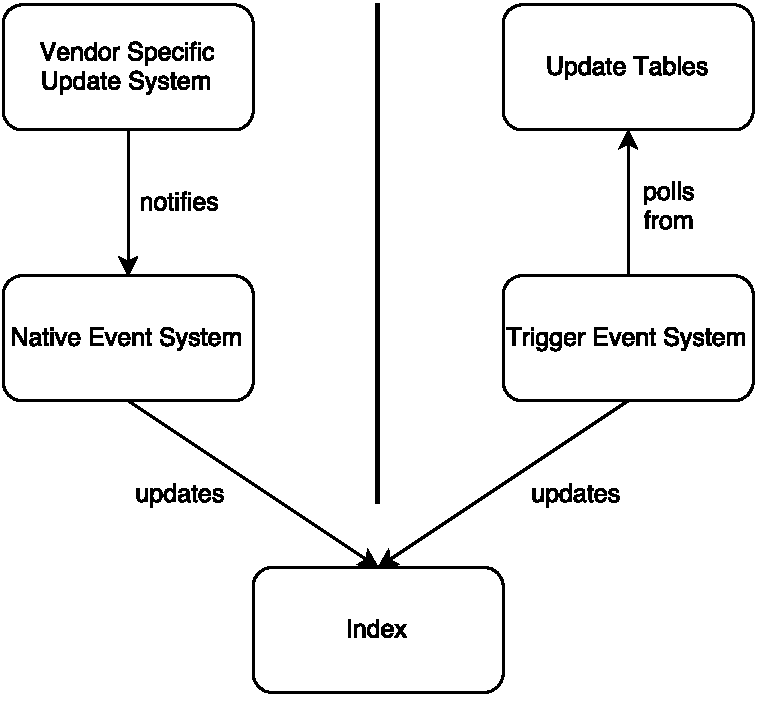
\includegraphics[scale=0.6]{images/UpdateConsumer_Architecture.pdf}
	\caption{Hibernate Search GenericJPA update mechanisms}
	\label{updateconsumer_architecture}
\end{figure}

\subsubsection{Additional work}
Since the native event system gets the proper information about changes from the vendor side, it doesn't require a lot of information about the general structure of the domain model and tables in the database. The Trigger based system however does need extra information as it has to poll info about changes from the database. This is the reason the user has to add this information as we have seen in chapter \ref{creating_the_tables}.

\pagebreak

\subsubsection{Features}
The native event system has the exact same updating behaviour as Hibernate Search ORM's update mechanism because it works on the same principles of using the existing event APIs. It just works for more ORM providers.
\\\\
With this similarity come two important drawbacks:
\begin{enumerate}
	\item It (the mechanism) only works with specifically supported JPA APIs
	\item Database changes coming from anything else than JPA APIs are not recognized and includes native SQL queries from EntityManagers. This also means that the database can only be used by the JPA application and no other programs should have write access to the database.
\end{enumerate}
\noindent
These two drawbacks are non-existent with the trigger event system as it doesn't require any specific JPA implementation (1) and works on the database level (2).

\pagebreak

\subsubsection{Summary}
The following table \ref{table:pros_and_cons_update_systems} summarizes all pros and cons - including the ones for being synchronous or asynchronous - once again:
\\
\begin{table}[h] 
	\centering
	\begin{tabular}{c||c|c}
		Approach & Pros & Cons \\ 
		\hline
		\hline
		\specialcell{Native \\ Event \\ System} & 
		\specialcell{+ no additional work \\ needed by the developer \\\\ + 100 \% up-to-date index \\ all the time} & 
		\specialcell{~\\- relies on different\\ implementation- \\ specific APIs \\ (only works with \\ specifically supported ones) \\\\
					- changes from outside\\ of the JPA provider \\are not recognized \\ (e.g. native SQL access)\\~} \\ 
		\hline
		\specialcell{Trigger \\ Event \\ System} & 
		\specialcell{~\\+ works with any JPA \\implementation \\ (even rarely used ones) \\\\
					+ changes from outside\\ of the JPA provider \\ are recognized \\ (e.g. native SQL access) \\~} & 
		\specialcell{- additional work by \\the developer needed \\ (annotations) \\\\ - unsuitable in \\ cases that need a \\ 100\% up-to-date index \\ all the time} \\ 
	\end{tabular}
	\footnotesize \caption{Pros and Cons of the two update systems}
	\label{table:pros_and_cons_update_systems}
\end{table}

\pagebreak
~
\pagebreak

\section{Usage of Hibernate Search GenericJPA} \label{usage_chapter}

Having described how Hibernate Search GenericJPA works and how it is designed we will now take a look at how it can be used in our example project from chapter \ref{example_project}. While having already explained this part by part in each chapter, the following is everything put together. For updating, we use the asynchronous updating mechanism as described in chapter \ref{async_approach}.

\subsection{Dependencies}

The following example needs to have at least these dependencies on the classpath:

\begin{enumerate}
	\item{EclipseLink 2.5.0}
	\item{HSQLDB 2.3.3 (in memory database)}
	\item{Hibernate Search GenericJPA}
\end{enumerate}

\pagebreak

\subsection{Entities}
First, we have to update the Entity mappings in the Java classes. We add the \textbf{@Indexed, @DocumentId, @Field, @IndexedEmbedded, @ContainedIn} as already known from the original Hibernate Search ORM (chapter \ref{setting_up_example_project}). Using Hibernate Search GenericJPA then requires us to add the @InIndex on every entity contained in the index as described in chapter \ref{using_hsearch_genericjpa_index}. Because we are using the asynchronous updating mechanism here, we have to add information about how to create the update tables as well (chapter \ref{creating_the_tables}).
\\\\
The resulting entities with the changes highlighted look like this:
\\
\lstset{language=java}
\lstset{moredelim=[is][\bfseries]{[*}{*]}}
\begin{lstlisting}[frame=htrbl, caption={Complete Book.java}, label={lst:book.java_complete}]
@Entity
@Table(name = "Book")
[*@InIndex*]
[*@Indexed*]
[*@UpdateInfo(tableName = "Book",
	idInfos = @IdInfo(
		columns = @IdColumn(
			column = "isbn",
			columnType = ColumnType.STRING)))*]
public class Book {
	
	@Id
	[*@DocumentId*]
	@Column(name = "isbn")
	private String isbn;
	
	@Column(name = "title")
	[*@Field*]
	private String title;
	
	@Column(name = "genre")
	[*@Field*]
	private String genre;
	
	@Lob
	@Column(name = "summary")
	[*@Field*]
	private String summary;
	
	@ManyToMany(mappedBy = "books", cascade = {
		CascadeType.MERGE,
		CascadeType.DETACH,
		CascadeType.PERSIST,
		CascadeType.REFRESH
	})
	[*@IndexedEmbedded(includeEmbeddedObjectId = true)*]
	private Set<Author> authors;
	
	// getters & setters ...
	
}
\end{lstlisting}

\lstset{language=java}
\lstset{moredelim=[is][\bfseries]{[*}{*]}}
\begin{lstlisting}[frame=htrbl, caption={Complete Author.java}, label={lst:author.java_complete}]
@Entity
@Table(name = "Author")
[*@InIndex*]
[*@UpdateInfo(tableName = "Author", 
	idInfos = @IdInfo(
		columns = @IdColumn(
			column = "authorId",
			columnType = ColumnType.LONG
	)
))*]
public class Author {
	
	@Id
	@GeneratedValue(strategy = GenerationType.AUTO)
	@Column(name = "authorId")
	[*@DocumentId*]
	private Long authorId;
	
	@Column(name = "firstName")
	[*@Field*]
	private String firstName;
	
	@Column(name = "lastName")
	[*@Field*]
	private String lastName;
	
	@Column(name = "country")
	[*@Field*]
	private String country;
	
	@ManyToMany(cascade = {
		CascadeType.MERGE,
		CascadeType.DETACH,
		CascadeType.PERSIST,
		CascadeType.REFRESH
	})
	@JoinTable(name = "Author_Book", 
		joinColumns = @JoinColumn(name = "authorFk", 
			referencedColumnName = "authorId"),
		inverseJoinColumns = @JoinColumn(name = "bookFk",
			referencedColumnName = "isbn"))
	[*@UpdateInfo(tableName = "Author_Book",
		idInfos = {
			@IdInfo(entity = Author.class,
				columns = @IdColumn(
				column = "authorFk",
				columnType = ColumnType.LONG)),
			@IdInfo(entity = Book.class,
				columns = @IdColumn(
				column = "bookFk",
				columnType = ColumnType.STRING))
	})*]
	[*@ContainedIn*]
	private Set<Book> books;
	
	// getters & setters ...
	
}
\end{lstlisting}


\pagebreak

\subsection{persistence.xml}

The persistence.xml file for our JPA based project is straightforward. As we are using an in-memory database with HSQLDB, settings for the schema creation and the user management are not important as the database is recreated at every restart.
\\

\lstset{language=xml}
\begin{lstlisting}[frame=htrbl, caption={Complete persistence.xml}, label={lst:persistence.xml_complete}]
<persistence xmlns="http://java.sun.com/xml/ns/persistence"
xmlns:xsi="http://www.w3.org/2001/XMLSchema-instance"
xsi:schemaLocation="http://java.sun.com/xml/ns/persistence
	http://java.sun.com/xml/ns/persistence/persistence_2_0.xsd"
	version="2.0">

	<persistence-unit name="EclipseLink_HSQLDB"
		transaction-type="RESOURCE_LOCAL">
		<provider>
			org.eclipse.persistence.jpa.PersistenceProvider
		</provider>
		<class>*.*.Author</class>
		<class>*.*.Book</class>
		<properties>
			<property name="javax.persistence.jdbc.driver"
				value="org.hsqldb.jdbcDriver"/>
			<property name="javax.persistence.jdbc.url"
				value="jdbc:hsqldb:mem:test"/>
			<property name="javax.persistence.jdbc.user"
				value="user"/>
			<property name="javax.persistence.jdbc.password"
				value="password"/>
			<property name="eclipselink.ddl-generation"
				value="drop-and-create-tables"/>
			<property name="eclipselink.logging.level"
				value="INFO"/>
			<property name="eclipselink.ddl-
				generation.output-mode"
				value="both"/>
		</properties>
	</persistence-unit>
	
</persistence>
\end{lstlisting}

\pagebreak
~
\pagebreak

\subsection{Code usage example}

In the following listing we show the whole lifecycle of a Hibernate Search GenericJPA based application. The relevant code passages are commented in the code.
\\

\lstset{language=java}
\lstset{moredelim=[is][\bfseries]{[*}{*]}}
\begin{lstlisting}[frame=htrbl, caption={Complete usage}, label={lst:complete_usage.java}]
Properties properties = new Properties();

// use the async backend
properties.setProperty(
	"hibernate.search.searchfactory.type",
	"sql"
);

// we are using HSQLDB, so use the right TriggerSource
properties.setProperty(
	"hibernate.search.trigger.source",
	"org.hibernate.search.genericjpa.db." + 
		"events.triggers.HSQLDBTriggerSQLStringSource"
);

// start up the EntityManagerFactory (entry-point to JPA)
// and create one EntityManager
EntityManagerFactory emf = Persistence
	.createEntityManagerFactory( "EclipseLink_HSQLDB" );
EntityManager em = emf.createEntityManager();

// start up Hibernate Search GenericJPA
JPASearchFactoryController searchController = 
	Setup.createSearchFactoryController( emf, properties );

// persist entities in the database
em.getTransaction().begin();
Author author = ...;
Book book = ...;
book.setAuthor( author );
em.persist( em );
em.getTransaction().commit();

// we are using an async backend, so wait a bit
// for the updating mechanism to handle the
// persist (Exception not handled here)
Thread.sleep( 10_000 );

// create a FullTextEntityManager
FullTextEntityManager fem = searchController
	.getFullTextEntityManager( em );

// query for all Books having the title "searchString"
FullTextQuery fullTextQuery = fem.createFullTextQuery(
	fem.getSearchFactory().buildQueryBuilder()
		.forEntity( Book.class )
		.get()
		.keyword()
		.onField( "title" )
		.matching( "searchString" )
		.createQuery(), 
	Book.class);

List<Book> books = (List<Book>) fullTextQuery.getResultList();

//handle the books
System.out.println( books );

// close everything 
// (FullTextEntityManager is not closed because
// the EntityManager is closed)
em.close();
searchController.close();
emf.close();
\end{lstlisting}
\noindent
Note that we didn't put the code into a main method. This is due to the fact that in a real application all this code would obviously not be put into one single method.
\\\\
The startup process of Hibernate Search GenericJPA is generally put into an extra lifecycle helper that stores a reference to the JPASearchFactoryController in a global variable upon application startup similar to what is generally done with JPA's EntityManagerFactory (at least in Java SE applications). All Search related code then acquires the reference to the JPASearchFactoryController from the global variable and uses it similarly to the above code. The lifecycle helper is also responsible for closing the JPASearchFactoryController when the application is shutting down.

\pagebreak

% !TeX spellcheck = en_GB

\section{Outlook}\label{outlook}

In this thesis we described how we can integrate Hibernate Search with JPA conform ORM implementations. We started by building a standalone integration of hibernate-search-engine, then integrated it with JPA and finally created an automatic index updating mechanism. All challenges described in chapter \ref{Challenges} have been resolved.
\\\\
The only feature needing some extra work is probably the generic updating mechanism with database triggers. At the moment the developer has to specify additional annotations containing information about the update tables by hand. As mentioned in chapter \ref{creating_the_tables}, at least some of the information is known to be able to be retrieved directly from JPA annotations. These mechanisms are not included in this thesis but can be added in a future version.
\\\\
During the process of designing and writing the code for Hibernate Search GenericJPA we tried to be as compatible with the orginal Hibernate Search API as possible. While one reason for this is to make the switch easier for developers that want to try it out, the biggest one is that the ultimate goal for this project is to be merged into the original Hibernate Search codebase even though we haven't mentioned this in the beginning.
\\\\
This is also why this project has to be looked as a proof of concept regardless of the fact that the code as it can be found on GitHub \footnote{Hibernate Search GenericJPA GitHub repository, see~\cite{hibernate_genericjpa_github}} can already be used in real applications. To make sure of this, every relevant part of Hibernate Search GenericJPA has been extensively tested in single feature-tests and integration-tests as described in chapter \ref{Methods}. Hibernate Search GenericJPA can therefore be considered stable. 
\\\\
The first steps of the merging process have already been discussed with the Hibernate Search development team and work on it is to be started in November 2015. This comes exactly at the right moment as the Hibernate Search team is planning API changes in the near future \footnote{Hibernate Search roadmap, see~\cite{hibernate_search_roadmap}} and some interfaces have to be altered (as seen in chapter \ref{integration_jpa}) in order to support generic JPA.
\\\\
As soon as the generic version is part of Hibernate Search and is fully compatible with its API, Hibernate Search could be looked at as a de-facto standard for fulltext search in JPA. Having such a standard would be quite beneficial for the JPA world as smaller JPA providers could have a better chance at getting a bigger user base, which is good for research and innovation.

\pagebreak
~


\onecolumn
% einfacher Zeilenabstand
\singlespacing
% Literaturliste soll im Inhaltsverzeichnis auftauchen
%\addcontentsline{toc}{section}{Literaturverzeichnis}
% Literaturverzeichnis anzeigen
%\renewcommand\refname{Literaturverzeichnis}
%\bibliography{Hauptdatei}

%% Index soll Stichwortverzeichnis heissen
% \newpage
% % Stichwortverzeichnis soll im Inhaltsverzeichnis auftauchen
% \addcontentsline{toc}{section}{Stichwortverzeichnis}
% \renewcommand{\indexname}{Stichwortverzeichnis}
% % Stichwortverzeichnis endgueltig anzeigen
% \printindex

\onehalfspacing

\newpage
\addcontentsline{toc}{section}{Used software}
\fancyhead[L]{Used Software}
\section*{Used software} \label{UsedSoftware}

\noindent
Github \\
IntelliJ IDEA

\pagebreak
~

% evtl. Anhang
\newpage
\addcontentsline{toc}{section}{Listings}
\fancyhead[L]{Listings} %Kopfzeile links
\section*{Listings}

Following are some interesting classes referenced in the thesis that were too long to fit into the text.
\\

\noindent
\textbf{Transaction}:\\
This class is the simple Transaction representation used to control index changes. It is not intended to be similar to a RDBMS transaction, but is merely a batch context with simple commit and rollback features.
\\
\lstset{language=java}
\begin{lstlisting}[frame=htrbl, caption={the simple Transaction contract}, label={lst:Transaction.java}]
public class Transaction implements TransactionContext {

	private boolean progress = true;
	private List<Synchronization> syncs = new ArrayList<>();
	
	@Override
	public boolean isTransactionInProgress() {
		return this.progress;
	}
	
	@Override
	public Object getTransactionIdentifier() {
		return this;
	}
	
	@Override
	public void registerSynchronization(
		Synchronization synchronization ) {
		this.syncs.add( synchronization );
	}
	
	/**
	 * @throws IllegalStateException if already commited/rolledback
	 */
	public void commit() {
		if ( !this.progress ) {
			throw new IllegalStateException( 
			"can't commit - " + 
			"No Search Transaction is in Progress!" );
		}
		this.progress = false;
		this.syncs.forEach( Synchronization::beforeCompletion );
		
		for ( Synchronization sync : this.syncs ) {
			sync.afterCompletion( Status.STATUS_COMMITTED );
		}
	}
	
	/**
	 * @throws IllegalStateException if already commited/rolledback
 	 */
	public void rollback() {
		if ( !this.progress ) {
			throw new IllegalStateException( 
			"can't rollback - " + 
			"No Search Transaction is in Progress!" );
		}
		this.progress = false;
		this.syncs.forEach( Synchronization::beforeCompletion );
	
		for ( Synchronization sync : this.syncs ) {
			sync.afterCompletion( Status.STATUS_ROLLEDBACK );
		}
	}

}
\end{lstlisting}

\pagebreak

\noindent
\textbf{StandaloneSearchConfiguration}:\\
hibernate-search-engine requires an object implementing the SearchConfiguration interface. StandaloneSearchConfiguration is the basic implementation of this used in our standalone version of Hibernate Search.
\\
\lstset{language=java}
\begin{lstlisting}[frame=htrbl, caption={StandaloneSearchConfiguration.java}, label={lst:StandaloneSearchConfiguration.java}]
/**
 * Manually defines the configuration. 
 * Classes and properties are the only implemented options at the moment.
 *
 * @author Martin Braun (adaption), Emmanuel Bernard
 */
public class StandaloneSearchConfiguration 
	extends SearchConfigurationBase 
	implements SearchConfiguration {

	private final Logger LOGGER = 
		Logger.getLogger( 
			StandaloneSearchConfiguration.class.getName() 
		);
		
	private final Map<String, Class<?>> classes;
	private final Properties properties;
	private final HashMap<Class<? extends Service>, Object> 
		providedServices;
	private final InstanceInitializer initializer;
	private SearchMapping programmaticMapping;
	private boolean transactionsExpected = true;
	private boolean indexMetadataComplete = true;
	private boolean idProvidedImplicit = false;
	private ClassLoaderService classLoaderService;
	private ReflectionManager reflectionManager;

	public StandaloneSearchConfiguration() {
		this( new Properties() );
	}

	public StandaloneSearchConfiguration(Properties properties) {
		this( 
			SubClassSupportInstanceInitializer.INSTANCE, 
			properties
		);
	}

	public StandaloneSearchConfiguration(InstanceInitializer init) {
		this( new Properties() );
	}

	public StandaloneSearchConfiguration(InstanceInitializer init, 
		Properties properties) {
		this.initializer = init;
		this.classes = new HashMap<>();
		this.properties = properties;
		// default values if nothing was explicitly set
		this.properties.computeIfAbsent(
			"hibernate.search.default.directory_provider", 
			(key) -> {
				LOGGER.info( 
				  "defaulting to RAM directory-provider" 
				);
			return "ram";
		});
		this.properties.computeIfAbsent(
			"hibernate.search.lucene_version", 
			(key) -> {
				LOGGER.info( 
					"defaulting to Lucene Version: " 
					+ Version.LUCENE_5_2_1.toString() 
				);
				return Version.LUCENE_5_2_1.toString();
		});
		this.reflectionManager = new JavaReflectionManager();
		this.providedServices = new HashMap<>();
		this.classLoaderService = new DefaultClassLoaderService();
	}

	public StandaloneSearchConfiguration addProperty(String key,
		String value) {
		properties.setProperty( key, value );
		return this;
	}

	public StandaloneSearchConfiguration addClass(Class<?> indexed) {
		classes.put( indexed.getName(), indexed );
		return this;
	}

	@Override
	public Iterator<Class<?>> getClassMappings() {
		return classes.values().iterator();
	}

	@Override
	public Class<?> getClassMapping(String name) {
		return classes.get( name );
	}

	@Override
	public String getProperty(String propertyName) {
		return properties.getProperty( propertyName );
	}

	@Override
	public Properties getProperties() {
		return properties;
	}

	@Override
	public ReflectionManager getReflectionManager() {
		return this.reflectionManager;
	}

	@Override
	public SearchMapping getProgrammaticMapping() {
		return programmaticMapping;
	}

	public StandaloneSearchConfiguration setProgrammaticMapping(
			SearchMapping programmaticMapping
		) {
		this.programmaticMapping = programmaticMapping;
		return this;
	}

	@Override
	public Map<Class<? extends Service>, Object> 
		getProvidedServices() {
		return providedServices;
	}

	public void addProvidedService(
			Class<? extends Service> serviceRole,
			Object service
		) {
		providedServices.put( serviceRole, service );
	}

	@Override
	public boolean isTransactionManagerExpected() {
		return this.transactionsExpected;
	}

	public void setTransactionsExpected(
			boolean transactionsExpected) {
		this.transactionsExpected = transactionsExpected;
	}

	@Override
	public InstanceInitializer getInstanceInitializer() {
		return initializer;
	}

	@Override
	public boolean isIndexMetadataComplete() {
		return indexMetadataComplete;
	}

	public void setIndexMetadataComplete(
		boolean indexMetadataComplete) {
		this.indexMetadataComplete = indexMetadataComplete;
	}

	@Override
	public boolean isIdProvidedImplicit() {
		return idProvidedImplicit;
	}

	public StandaloneSearchConfiguration 
		setIdProvidedImplicit(boolean idProvidedImplicit) {
		this.idProvidedImplicit = idProvidedImplicit;
		return this;
	}

	@Override
	public ClassLoaderService getClassLoaderService() {
		return classLoaderService;
	}

	public void setClassLoaderService(
		ClassLoaderService ) {
		this.classLoaderService = classLoaderService;
	}

}
\end{lstlisting}

\pagebreak

\noindent
\textbf{BasicEntityProvider}:\\
This is the basic implementation of the EntityProvider interface which is used to abstract the database access in the standalone version. It uses a JPA EntityManager to accomplish this.
\\
\lstset{language=java}
\begin{lstlisting}[frame=htrbl, caption={BasicEntityProvider.java}, label={lst:BasicEntityProvider.java}]
public class BasicEntityProvider implements EntityProvider {

	private static final String QUERY_FORMAT = 
		"SELECT obj FROM %s obj " +
		"WHERE obj.%s IN :ids";
	private final EntityManager em;
	private final Map<Class<?>, String> idProperties;

	public BasicEntityProvider(EntityManager em,
		Map<Class<?>, String> idProperties) {
		this.em = em;
		this.idProperties = idProperties;
	}

	@Override
	public void close() throws IOException {
		this.em.close();
	}

	@Override
	public Object get(Class<?> entityClass, Object id,
		Map<String, String> hints) {
		return this.em.find( entityClass, id );
	}

	@SuppressWarnings({"rawtypes", "unchecked"})
	@Override
	public List getBatch(Class<?> entityClass, List<Object> ids,
		Map<String, String> hints) {
		List<Object> ret = new ArrayList<>( ids.size() );
		if ( ids.size() > 0 ) {
			String idProperty = 
				this.idProperties.get( entityClass );
			String queryString = 
				String.format(
					QUERY_FORMAT,
					this.em.getMetamodel()
						.entity( entityClass )
						.getName(),
					idProperty
		);
		Query query = this.em.createQuery( queryString );
		query.setParameter( "ids", ids );
			ret.addAll( query.getResultList() );
		}
		return ret;
	}
	
	public void clearEm() {
		this.em.clear();
	}

	public EntityManager getEm() {
		return this.em;
	}

}
\end{lstlisting}

\pagebreak

\noindent
\textbf{Obtaining the idProperties}:\\
This code snippet shows how the idProperties map needed for the instantiation of a BasicEntityProvider can be obtained. This mechanism is used on some other places of Hibernate Search GenericJPA as well.
\\
\lstset{language=java}
\begin{lstlisting}[frame=htrbl, caption={Obtaining idProperties}, label={lst:idProperties.java}]
SearchConfiguration config = ...;

MetadataProvider metadataProvider = 
	MetadataUtil.getDummyMetadataProvider( config );
MetadataRehasher rehasher = new MetadataRehasher();

List<RehashedTypeMetadata> rehashedTypeMetadatas = new ArrayList<>();
for ( Class<?> indexRootType : this.getIndexRootTypes() ) {
	RehashedTypeMetadata rehashed = 
		rehasher.rehash( 
			metadataProvider
				.getTypeMetadataFor( indexRootType ) 
		);
	rehashedTypeMetadatas.add( rehashed );
}

Map<Class<?>, String> idProperties = 
	MetadataUtil.calculateIdProperties( rehashedTypeMetadatas );
\end{lstlisting}

\pagebreak

\noindent
\textbf{MultiQueryAccess}:\\
This is the utility class used to scroll results from multiple queries at once while retrieving the events from the database in the asynchronous approach.
\\
\lstset{language=java}
\begin{lstlisting}[frame=htrbl, caption={MultiQueryAccess.java}, label={lst:MultiQueryAccess.java}]
/**
 * Utility class that allows you to access multiple JPA queries at once.
 * Data is retrieved from the database in batches
 * and ordered by a given comparator.
 * No need for messy Unions on the database level! <br>
 * <br>
 * This is particularly useful if you scroll all the data 
 * from the database incrementally and if you can 
 * compare in Code.
 *
 * @author Martin
 */
public class MultiQueryAccess {

	private final Map<String, Long> currentCountMap;
	private final Map<String, Query> queryMap;
	private final Comparator<ObjectIdentifierWrapper> comparator;
	private final int batchSize;
	
	private final Map<String, Long> currentPosition;
	private final Map<String, LinkedList<Object>> values;
	
	private Object scheduled;
	private String identifier;


	public MultiQueryAccess(
		Map<String, Long> countMap,
		Map<String, Query> queryMap,
		Comparator<ObjectIdentifierWrapper> comparator,
		int batchSize) {
		if ( countMap.size() != queryMap.size() ) {
			throw new IllegalArgumentException( 
				"countMap.size() must be equal " + 
					"to queryMap.size()" );
		}
		this.currentCountMap = countMap;
		this.queryMap = queryMap;
		this.comparator = comparator;
		this.batchSize = batchSize;
		this.currentPosition = new HashMap<>();
		this.values = new HashMap<>();
		for ( String ident : queryMap.keySet() ) {
			this.values.put( ident, new LinkedList<>() );
			this.currentPosition.put( ident, 0L );
		}
	}

	private static int toInt(Long l) {
		return (int) (long) l;
	}

	/**
	 * increments the value to be returned by {@link #get()}
	 *
	 * @return true if there is a value left to be visited 
	 *	in the database
	 */
	public boolean next() {
	
	/*
	 *
	 *
	 * indentation broken to make this readable
	 *
	 *
	 */
	
this.scheduled = null;
this.identifier = null;
List<ObjectIdentifierWrapper> tmp =
	new ArrayList<>( this.queryMap.size() );

for ( Map.Entry<String, Query> entry : this.queryMap.entrySet() ) {
	String identifier = entry.getKey();
	Query query = entry.getValue();
	if ( !this.currentCountMap.get( identifier ).equals( 0L ) ) {
		if ( this.values.get( identifier ).size() == 0 ) {
			// the last batch is empty. get a new one
			Long processed = 
				this.currentPosition.get( identifier );
			// yay JPA...
			query.setFirstResult( toInt( processed ) );
			query.setMaxResults( this.batchSize );
			@SuppressWarnings("unchecked")
			List<Object> list = query.getResultList();
			this.values.get( identifier ).addAll( list );
		}
		Object val = this.values.get( identifier ).getFirst();
		tmp.add( new ObjectIdentifierWrapper( val, identifier ) );
	}
}
tmp.sort( this.comparator );
if ( tmp.size() > 0 ) {
	ObjectIdentifierWrapper arr = tmp.get( 0 );
	this.scheduled = arr.object;
	this.identifier = arr.identifier;
	this.values.get( this.identifier ).pop();
	Long currentPosition = this.currentPosition.get( arr.identifier );
	Long newCurrentPosition = 
		this.currentPosition
			.computeIfPresent( arr.identifier, 
				(clazz, old) -> old + 1 );
	if ( Math.abs( newCurrentPosition - currentPosition ) != 1L ) {
		throw new AssertionFailure( 
			"the new currentPosition count " + 
			"should be exactly 1 " +
			"greater than the old one" );
	}
	Long count = this.currentCountMap.get( arr.identifier );
	Long newCount = this.currentCountMap.computeIfPresent(
		arr.identifier, (clazz, old) -> old - 1
	);
	if ( Math.abs( count - newCount ) != 1L ) {
		throw new AssertionFailure( 
			"the new old remaining count " + 
				should be exactly 1 " +
				"greater than the new one" );
	}
}
return this.scheduled != null;
}

	/**
	* @return the current value
	*/
	public Object get() {
		if ( this.scheduled == null ) {
			throw new IllegalStateException(
				"either empty or next() has " + 
					"not been called" );
		}
		return this.scheduled;
	}

	/**
	* @return the identifier of the current value
	*/
	public String identifier() {
		if ( this.identifier == null ) {
			throw new IllegalStateException( 
				"either empty or next() has " + 
					"not been called" );
		}
		return this.identifier;
	}

	public static class ObjectIdentifierWrapper {
	
		public final Object object;
		public final String identifier;
		
		public ObjectIdentifierWrapper(Object object,
			String identifier) {
			this.object = object;
			this.identifier = identifier;
		}
	
	}

}
\end{lstlisting}

\pagebreak

~

\newpage
\addcontentsline{toc}{section}{Tables}
\fancyhead[L]{Tables}
\section*{Tables}
This section contains all tables referenced in this thesis.
\\

\noindent
\textbf{JPASearchFactoryController configuration}:\\
When instantiating the JPASearchFactoryController with the Setup class the developer has to pass a property-Map (or a Java Properties) object. Besides containing the hibernate-search-engine configuration properties, some Hibernate Search GenericJPA configuration properties can be set in this map as well:
\\
\begin{table}[h] 
	\centering
	\begin{tabular}{|c|c|}
		\hline 
		hibernate.search.useJTATransactions & \specialcell{ \textbf{false} \\ true } \\ 
		\hline 
		hibernate.search.searchfactory.type & \specialcell{ \textbf{sql} \\ manual-updates  \\ eclipselink \\ hibernate \\ openjpa} \\ 
		\hline
		hibernate.search.trigger.batchSizeForUpdates & \specialcell{ \textbf{5} } \\
		\hline
		hibernate.search.trigger.batchSizeForUpdateQueries & \specialcell{ \textbf{20} } \\
		\hline
		hibernate.search.trigger.updateDelay & \specialcell{ \textbf{200} } \\
		\hline
		hibernate.search.trigger.source & \specialcell{ <class> } \\
		\hline
		hibernate.search.additionalIndexedTypes & \specialcell{ <class>,<class>,... } \\
		\hline
		hibernate.search.transactionManagerProvider & \specialcell{
			\textbf{org.hibernate.}\\\textbf{search.generic}\\\textbf{jpa.trans}\\\textbf{action.impl}\\
			\textbf{JNDILookup}\\\textbf{Transaction}\\\textbf{ManagerProvider} 
		} \\
		\hline
		hibernate.search.transactionManagerProvider.jndi & \specialcell{ <jndi-string> } \\
		\hline
		hibernate.search.trigger.createstrategy & \specialcell{
			\textbf{create} \\
			create-drop \\
			dont-create
		} \\
		\hline
	\end{tabular}
	\footnotesize \caption{Basic JPASearchFactoryController configuration properties (\textbf{default})}
	\label{table:config_properties_jpasearchfactorycontroller}
\end{table}

\pagebreak
~

\newpage
\addcontentsline{toc}{section}{References}
\fancyhead[L]{References}
%
% ---- Bibliography ----
%
\begin{thebibliography}{100}
	
	\bibitem{jsr_jpa1} JSR 220: Enterprise Java Beans 3.0
	\url{https://jcp.org/en/jsr/detail?id=220}, 09/09/2015
	%
	
	\bibitem{javaworld_jpa1} Javaworld: Understanding JPA, Part 1
	\url{http://www.javaworld.com/article/2077817/java-se/understanding-jpa-part-1-the-object-oriented-paradigm-of-data-persistence.html}, 09/09/2015
	
	\bibitem{hibernate_orm} Hibernate ORM project homepage
	\url{http://hibernate.org/orm/}, 09/09/2015
	
	\bibitem{hibernate_search_homepage} Hibernate Search project homepage
	\url{http://hibernate.org/search/}, 09/09/2015
	
	\bibitem{hsearch_source_code_git} Hibernate Search GitHub repository
	\url{https://github.com/hibernate/hibernate-search}, 09/09/2015
	
	\bibitem{hibernate_search_faq} Hibernate Search FAQ
	\url{http://hibernate.org/search/faq/}, 09/09/2015
	
	\bibitem{lucene_apache_org} Lucene Website
	\url{https://lucene.apache.org/core/}, 09/09/2015
	
	\bibitem{elasticsearch_java_api} ElasticSearch Java API
	\url{https://www.elastic.co/guide/en/elasticsearch/client/java-api/current/index.html}, 09/09/2015
	
	\bibitem{solr_java_api} Solr Java API
	\url{https://wiki.apache.org/solr/Solrj}, 09/09/2015
	
	\bibitem{xkcd_competing_standards_source} xkcd \#927 on competing standards
	\url{https://xkcd.com/927/}, 09/09/2015
	
	\bibitem{top_down_strandh} Top-down programming, Robert Strandh
	\url{http://dept-info.labri.fr/~strandh/Teaching/PFS/Common/Strandh-Tutorial/top-down-programming.html},
	09/09/2015
	
	\bibitem{bottom_up_strandh} Bottom-up programming, Robert Strandh
	\url{http://dept-info.labri.fr/~strandh/Teaching/PFS/Common/Strandh-Tutorial/bottom-up-programming.html},
	09/09/2015
	
	\bibitem{singleresponsibility_objectmentor} objectmentor.com: Article on Single Responsibility Principle
	\url{http://www.objectmentor.com/resources/articles/srp.pdf}, 09/09/2015
	
	\bibitem{openclosed_objectmentor} objectmentor.com: Article on Open-Closed-Principle
	\url{http://www.objectmentor.com/resources/articles/ocp.pdf}, 09/09/2015
	
	\bibitem{openclosed_bertrand} Object-Oriented Software Construction, Prentice Hall, 1988, Bertrand Meyer
	
	\bibitem{maven_homepage} Maven project homepage
	\url{https://maven.apache.org/}, 09/09/2015
	
	\bibitem{jdbc_oracle} Oracle JDBC overview
	\url{http://www.oracle.com/technetwork/java/javase/jdbc/index.html}, 09/09/2015
	
	\bibitem{oledb_ms} Documentation on how to use OleDb with .NET
	\url{https://msdn.microsoft.com/en-us/library/5ybdbtte(v=vs.71).aspx}, 09/09/2015
	
	\bibitem{wikibooks_on_jpa} Wikibooks on Java Persistence
	\url{https://en.wikibooks.org/wiki/Java_Persistence/What_is_JPA\%3F}, 09/09/2015
	
	\bibitem{stackoverflow_jpa} Stackoverflow JPA tag
	\url{http://stackoverflow.com/tags/jpa/info}, 09/09/2015
	
	\bibitem{hibernate_ogm} Hibernate OGM project homepage
	\url{http://hibernate.org/ogm/}, 09/09/2015
	
	\bibitem{eclipselink} EclipseLink project homepage
	\url{http://www.eclipse.org/eclipselink/}, 09/09/2015
	
	\bibitem{jpa_21_jcp} JSR 338: JPA 2.1 specification
	\url{https://jcp.org/en/jsr/detail?id=338}, 09/09/2015
	
	\bibitem{openjpa} OpenJPA project homepage
	\url{http://openjpa.apache.org/}, 09/09/2015
	
	\bibitem{java_ee_spec} Java EE specification on oracle.com
	\url{http://www.oracle.com/technetwork/java/javaee/tech/index.html}, 09/09/2015
	
	\bibitem{sql_like_w3schools} w3schools on SQL LIKE
	\url{http://www.w3schools.com/sql/sql_like.asp}, 09/09/2015
	
	\bibitem{lucene_basic_concepts} Lucene Tutorial
	\url{http://www.lucenetutorial.com/basic-concepts.html}, 09/09/2015
	
	\bibitem{elasticsearch_homepage} ElasticSearch Homepage
	\url{https://www.elastic.co/products/elasticsearch}, 09/09/2015
	
	\bibitem{solr_homepage} Solr Homepage
	\url{http://lucene.apache.org/solr/}, 09/09/2015
	
	\bibitem{elasticsearch_downloads_website} ElasticSearch Download website
	\url{https://www.elastic.co/downloads/elasticsearch}, 09/09/2015
	
	\bibitem{solr_security} Solr security
	\url{https://wiki.apache.org/solr/SolrSecurity}, 09/09/2015
	
	\bibitem{elasticsearch_security} elastic Shield (security for ElasticSearch)
	\url{https://www.elastic.co/products/shield}, 09/09/2015
	
	\bibitem{solr_admin} Solr Administration (Core Specific Tools)
	\url{https://cwiki.apache.org/confluence/display/solr/Core-Specific+Tools}, 09/09/2015
	
	\bibitem{elasticsearch_admin} ElasticHQ
	\url{http://www.elastichq.org/}, 09/09/2015
	
	\bibitem{elasticsearch_clustering} ElasticSearch: Life inside a cluster
	\url{https://www.elastic.co/guide/en/elasticsearch/guide/current/distributed-cluster.html}, 09/09/2015
	
	\bibitem{solr_clustering} Solr: Introduction to Scaling and Distribution
	\url{https://cwiki.apache.org/confluence/display/solr/Introduction+to+Scaling+and+Distribution}, 09/09/2015
	
	\bibitem{hibernate_search_engine_mvnrepository} hibernate-search-engine on mvnrepository.org
	\url{http://mvnrepository.com/artifact/org.hibernate/hibernate-search-engine/5.4.0.Final}, 09/09/2015
	
	\bibitem{hibernate_search_roadmap} Hibernate Search roadmap
	\url{http://hibernate.org/search/roadmap/}, 09/09/2015
	
	\bibitem{hibernate_search_javadoc} Hibernate Search JavaDoc
	\url{https://docs.jboss.org/hibernate/search/5.5/api/}, 09/09/2015
	
	\bibitem{hibernate_search_doc} Hibernate Search documentation
	\url{http://hibernate.org/search/documentation/}, 09/09/2015
	
	\bibitem{hibernate_search_doc_massindexer} Hibernate Search documentation (MassIndexer, v5.4)
	\url{https://docs.jboss.org/hibernate/search/5.4/reference/en-US/html_single/#search-batchindex-massindexer}, 09/09/2015
	
	\bibitem{mysql_developers_lib} MySQL - Developer's Library, Fourth Edition, 2009, Paul DuBois
	
	\bibitem{postgres_triggers} CREATE TRIGGER in PostgreSQL
	\url{http://www.postgresql.org/docs/9.1/static/sql-createtrigger.html}, 09/09/2015
	
	\bibitem{hsqldb_triggers} Triggers in HSQLDB
	\url{http://hsqldb.org/doc/guide/triggers-chapt.html}, 09/09/2015
	
	\bibitem{firebird_triggers} Triggers in Firebird
	\url{http://www.firebirdsql.org/refdocs/langrefupd21-ddl-trigger.html}, 09/09/2015
	
	\bibitem{postgres_truncate} Truncate statement PostgreSQL docs
	\url{http://www.postgresql.org/docs/9.1/static/sql-truncate.html}, 09/09/2015
	
	\bibitem{firebird_conformance} Firebird conformance
	\url{http://www.firebirdsql.org/en/sql-conformance/}, 09/09/2015
	
	\bibitem{hibernate_genericjpa_github} Hibernate Search GenericJPA GitHub repository
	\url{https://github.com/Hotware/Hibernate-Search-GenericJPA}, 09/09/2015
	
	
\end{thebibliography}

%\newpage
% Erklärung
%\addcontentsline{toc}{section}{Erklärung}
%\fancyhead[L]{Erklärung}
%\section*{Erklärung}

\begin{verbatim}

\end{verbatim}

\noindent
\begin{LARGE}Erklärung zur Bachelorarbeit\end{LARGE}
\begin{verbatim}


\end{verbatim}
Ich versichere, die von mir vorgelegte Arbeit selbstständig verfasst zu haben. Alle Stellen, die wörtlich oder sinngemäß aus veröffentlichten oder nicht veröffentlichten Arbeiten anderer entnommen sind, habe ich als entnommen kenntlich gemacht. Sämtliche Quellen und Hilfsmittel, die ich für die Arbeit benutzt habe, sind angegeben. Die Arbeit hat mit gleichem Inhalt bzw. in wesentlichen Teilen noch keiner anderen Prüfungsbehörde vorgelegen.



\begin{displaymath}
% use packages: array
\begin{array}{ll}
Unterschrift:~~~~~~~~~~~~~~~~~~~~~~~~~~~~~~~~~~~~~~~~~~
& Ort, Datum:~~~~~~~~~~~~~~~~~~~~~~~~~~~~~~~~~~~~~~~~~~
\end{array}
\end{displaymath}


% leere Abschlussseite
\newpage
\thispagestyle{empty} % erzeugt Seite ohne Kopf- / Fusszeile
\section*{ }

\end{document}